\chapter{Testing}
\label{chap:testing}
Now I have designed the algorithms and developed the code. I can flash the microcontroller chip with the program. To do this, I will first need to compile the assembly language program into \verb|.hex| format which can be programmed onto it. \newline
\begin{figure}[H]
    \centering
    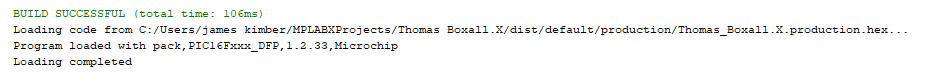
\includegraphics[width=0.9\textwidth]{images/compileSuccessful.png}
    \caption{Screenshot of MPLABX showing my code successfully compiling}
    \label{fig:compileSuccessful}
\end{figure}
\noindent After constructing the circuit as specified in my circuit design (\textit{Appendix \ref{chap:schematic})}, I connected the breadboard to power and let the program run \newline
This didn't work at first. After some troubleshooting, I realised that the problem was within the \verb|waitFiveSecondsCheckButton| subroutine. To fix this, I replaced it with a new subroutine, which only waited for one second, this mitigated the need for a second loop as I was only looping to 100, rather than 100 and 5 in two separate loops. This does increase the size of my program as I have to call the same function five times to achieve the same wait time as I would for the five second subroutine. This worked first time, and the microcontroller cycled through the traffic light sequence perfect first time. \newline
Now that the traffic lights are working, I am able to check if the pedestrian crossing is working and triggering correctly. To test this, I can press the button while the traffic lights are in a random state and observe the outcome. This worked first time, with the white wait LED turning on as soon as the button was pressed then when the current set of traffic lights reached the end of their sequence, the pedestrian crossing cycled as laid out in the design. The timings felt extremely out of proportion, so I reduced the crossing time to 3 seconds, this made the pedestrian crossing time feel better.
\begin{figure}[H]
    \centering
    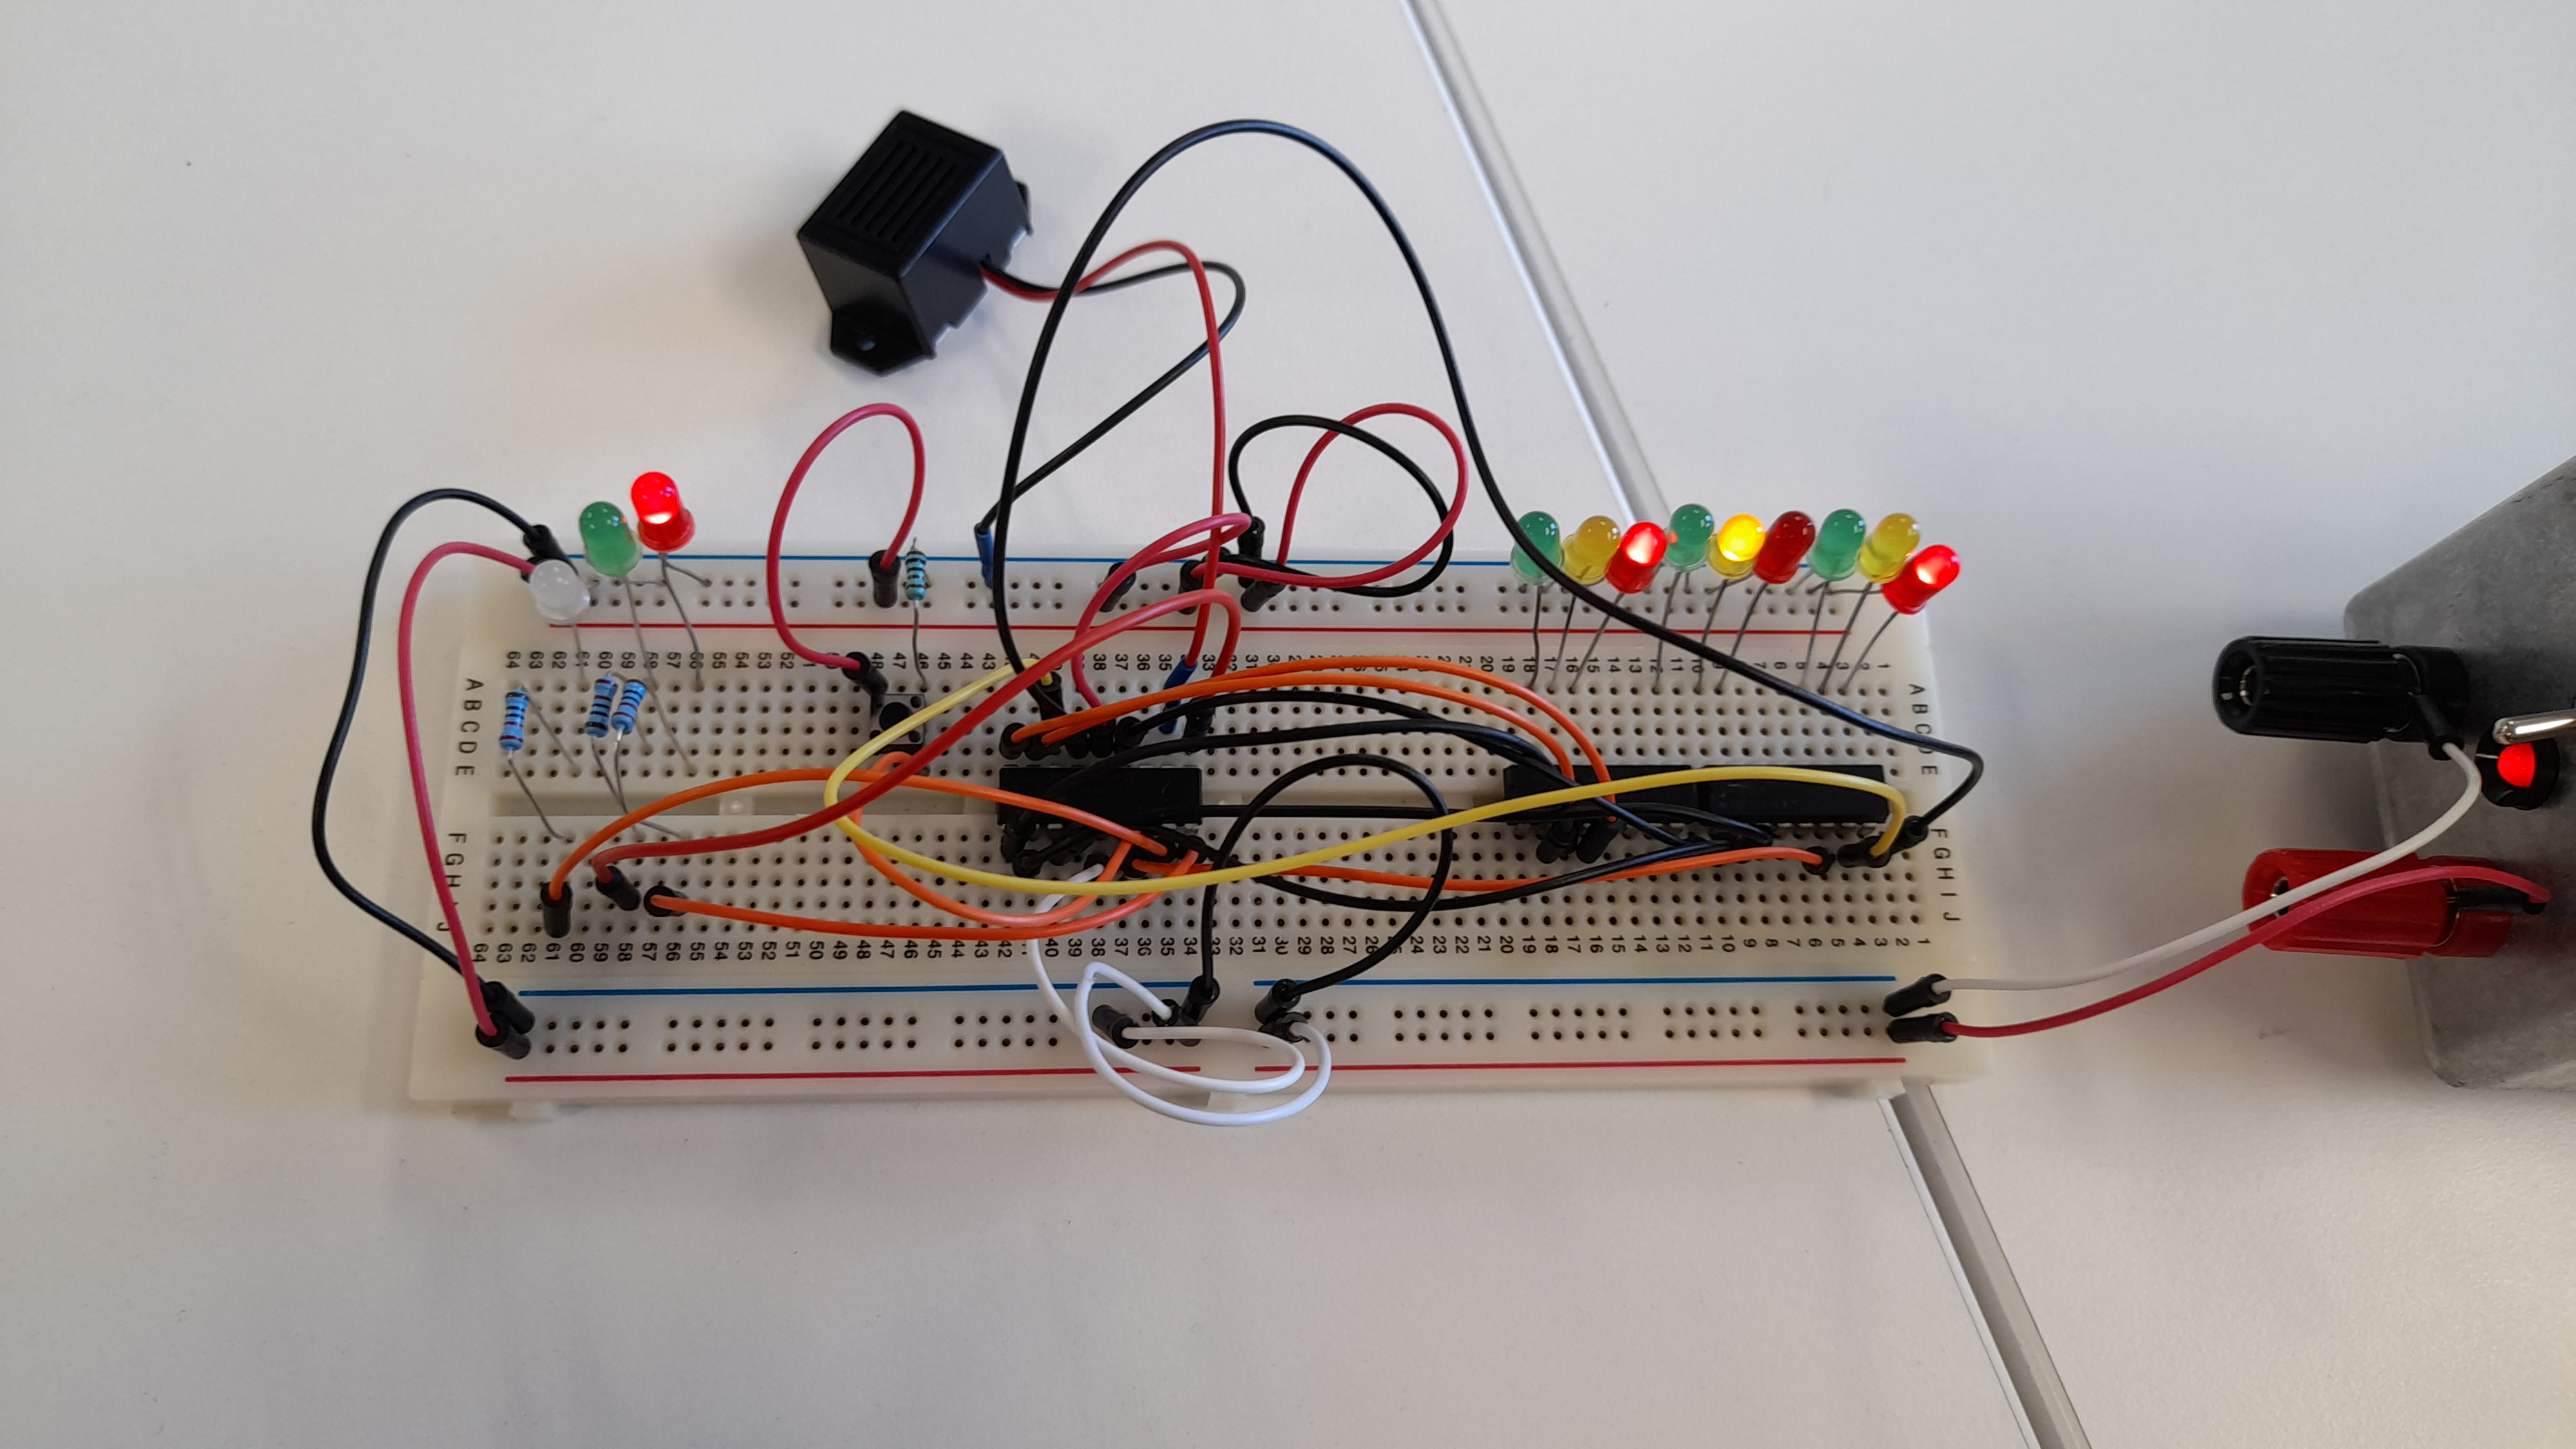
\includegraphics[width=0.9\textwidth]{images/unneatened.jpg}
    \caption{Circuit connected with temporary jumper wires}
    \label{fig:unneatened}
\end{figure}
\noindent This means that I have now completed construction of the system. I will now need to neaten the circuit.


\section{Sequence testing}
There are two different sets of sequences which I will need to check. One being the traffic light sequence and the other being the pedestrian crossing sequence.
\subsection{Traffic Lights sequence}
\begin{figure}[H]
    \begin{minipage}{0.45\textwidth}
        \centering
        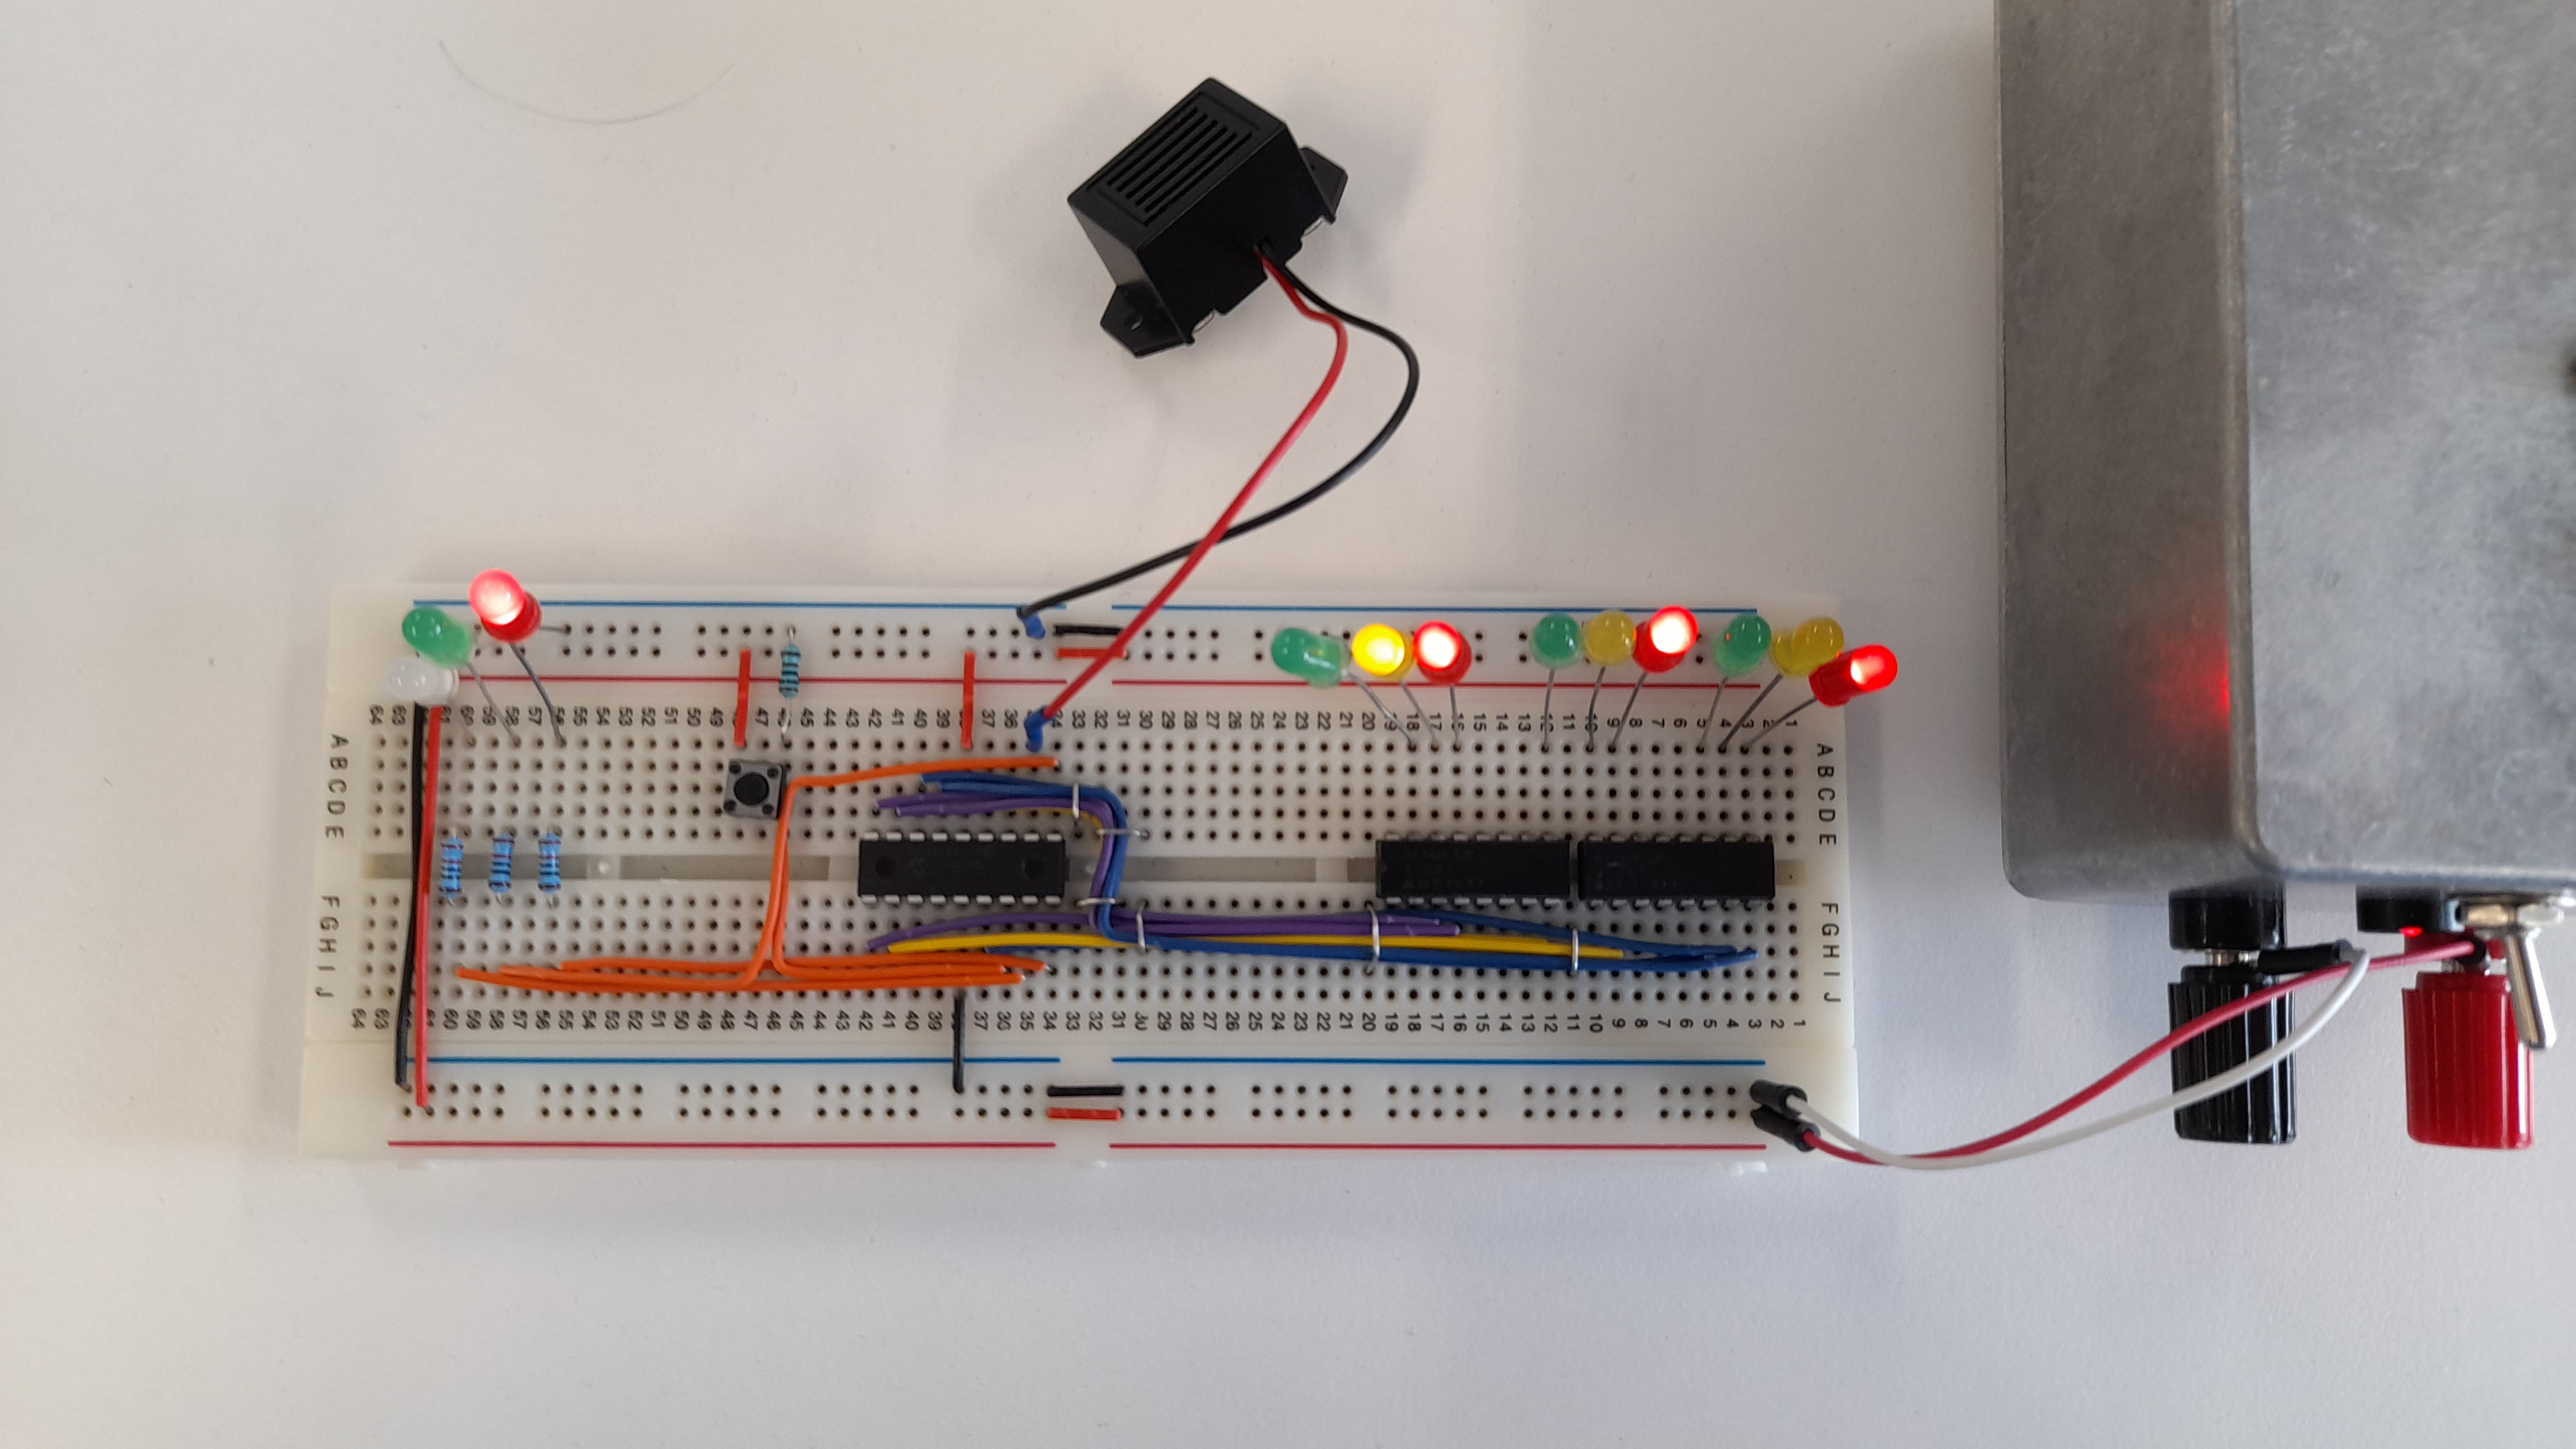
\includegraphics[width=0.9\textwidth]{images/final-testing/state_1.jpg}
        \caption{State 1 - pink traffic lights in red and amber phase}
        \label{fig:state_1}
    \end{minipage}\hfill
    \begin{minipage}{0.45\textwidth}
        \centering
        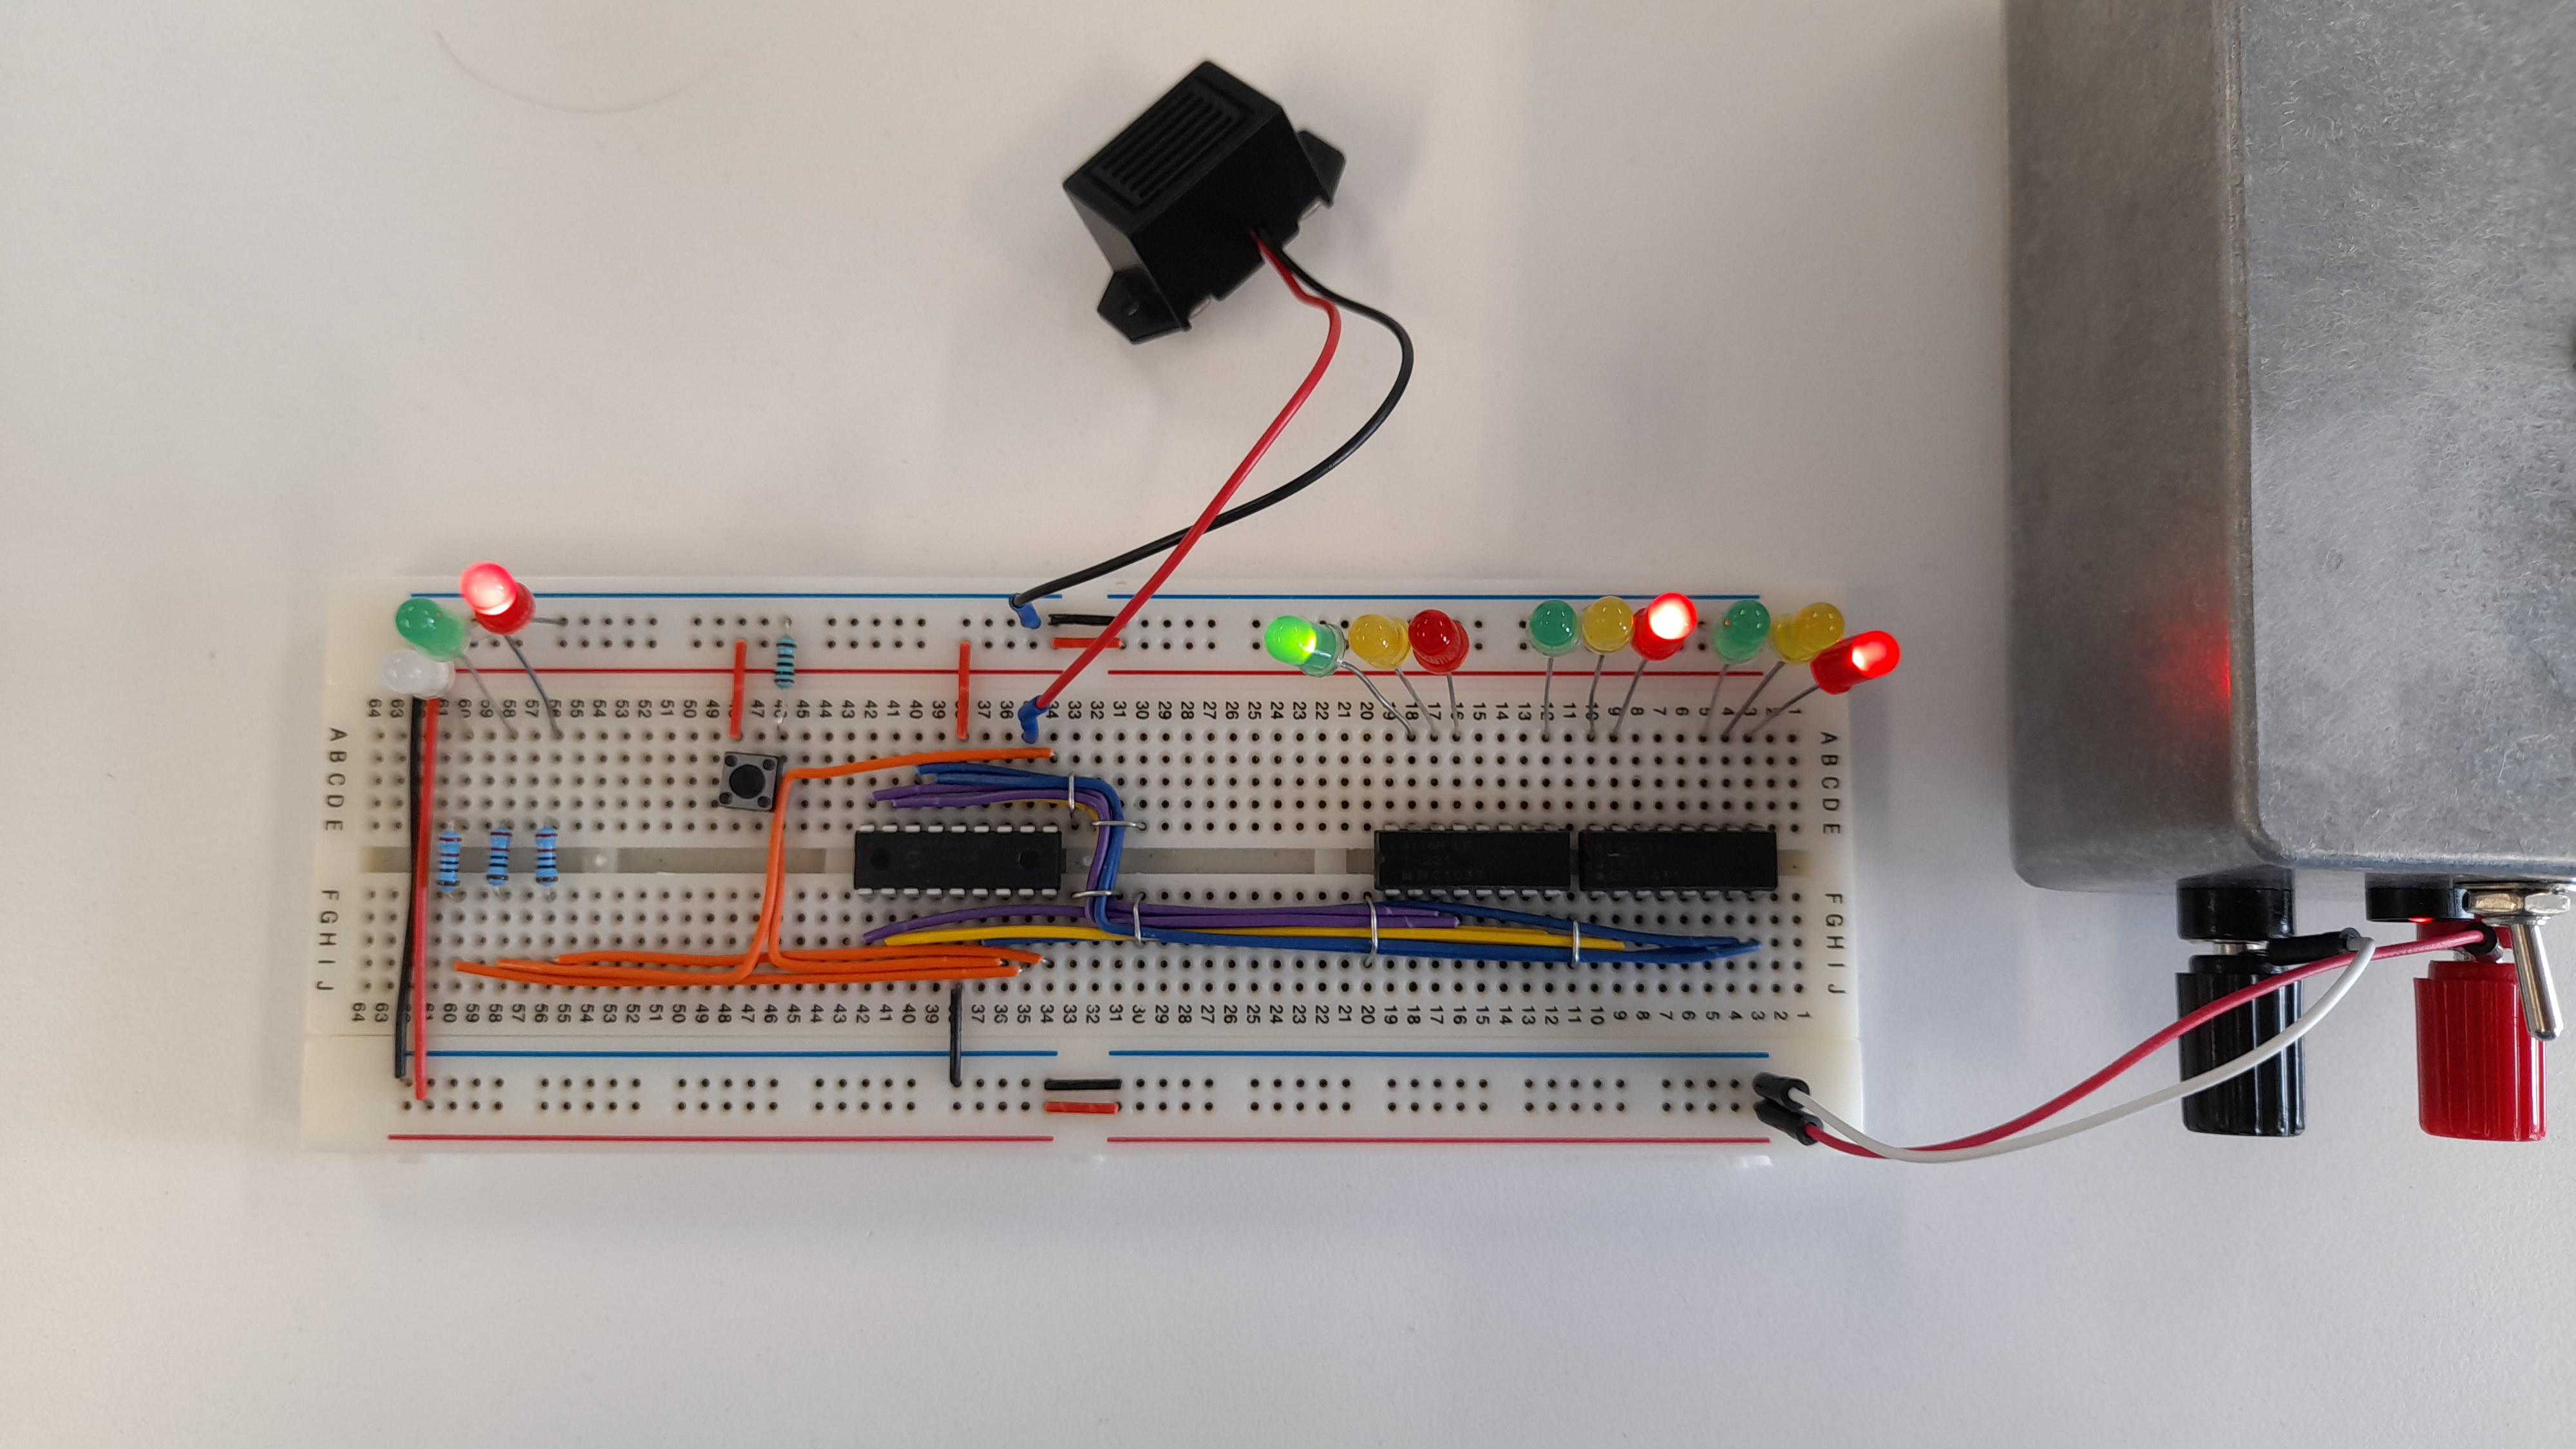
\includegraphics[width=0.9\textwidth]{images/final-testing/state_2.jpg}
        \caption{State 2 - pink traffic lights in green phase}
        \label{fig:state_2}
    \end{minipage}
\end{figure}
\begin{figure}[H]
    \begin{minipage}{0.45\textwidth}
        \centering
        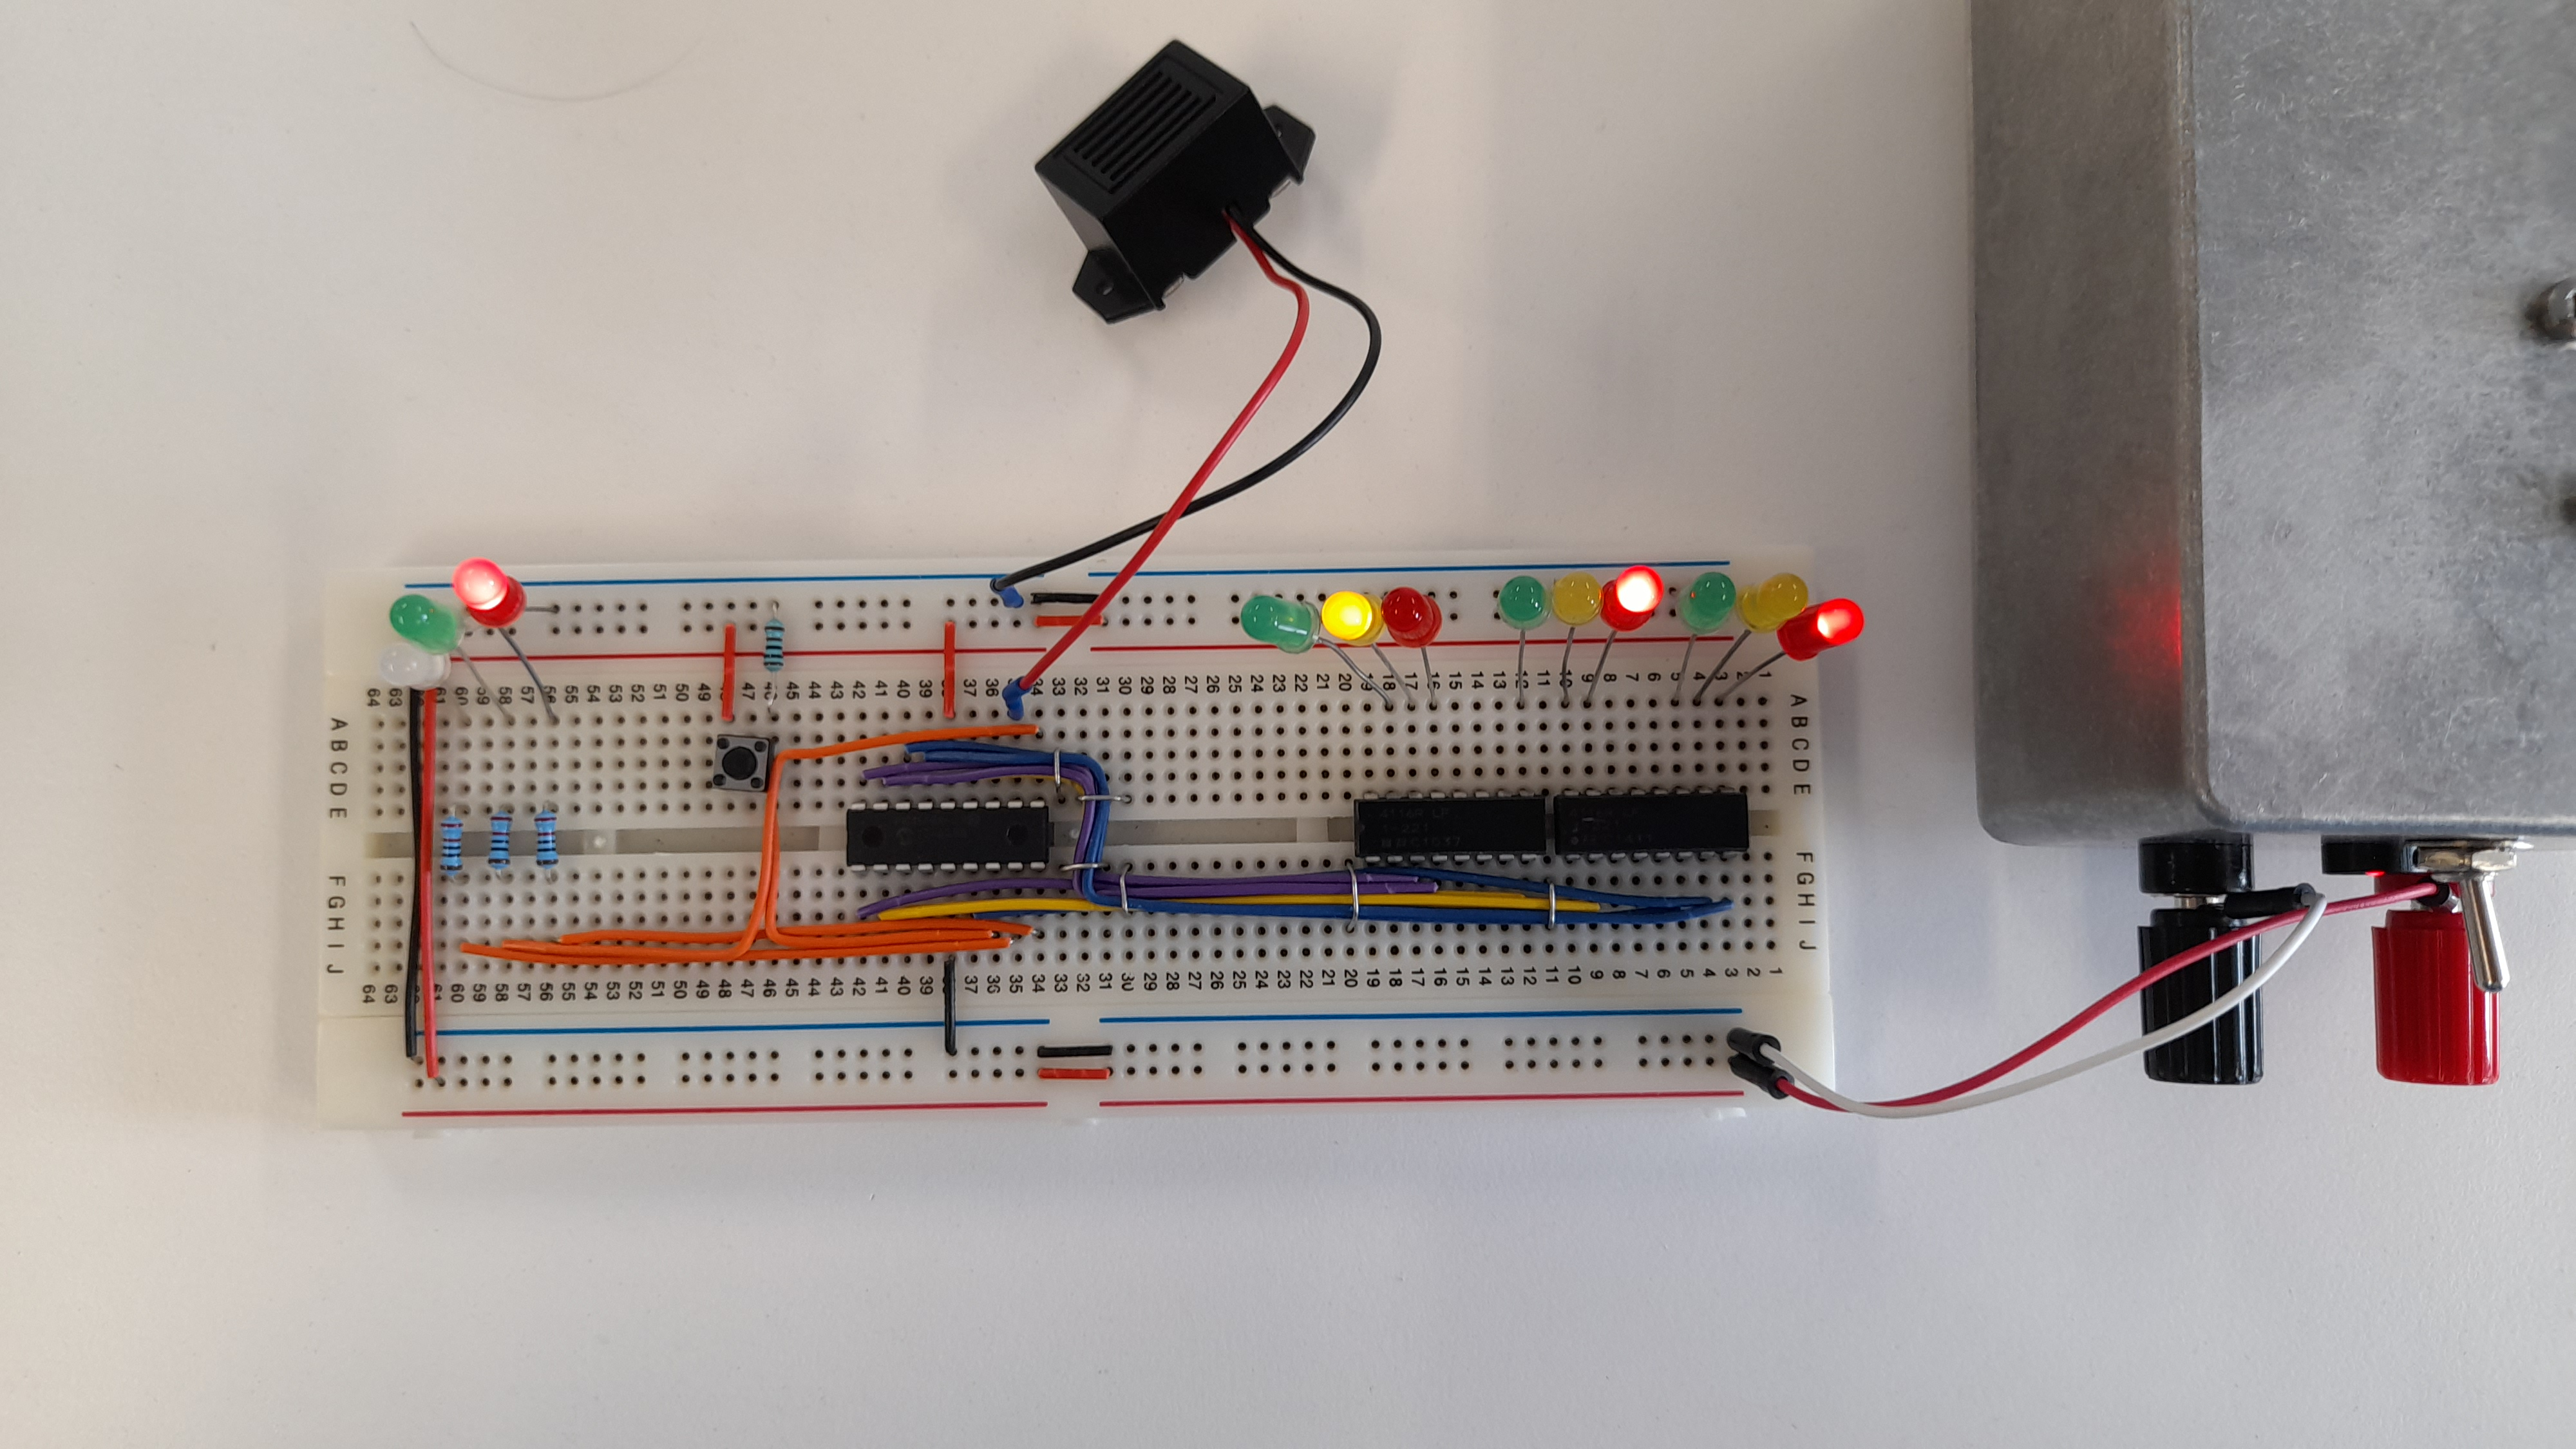
\includegraphics[width=0.9\textwidth]{images/final-testing/state_3.jpg}
        \caption{State 3 - pink traffic lights in amber phase}
        \label{fig:state_3}
    \end{minipage}\hfill
    \begin{minipage}{0.45\textwidth}
        \centering
        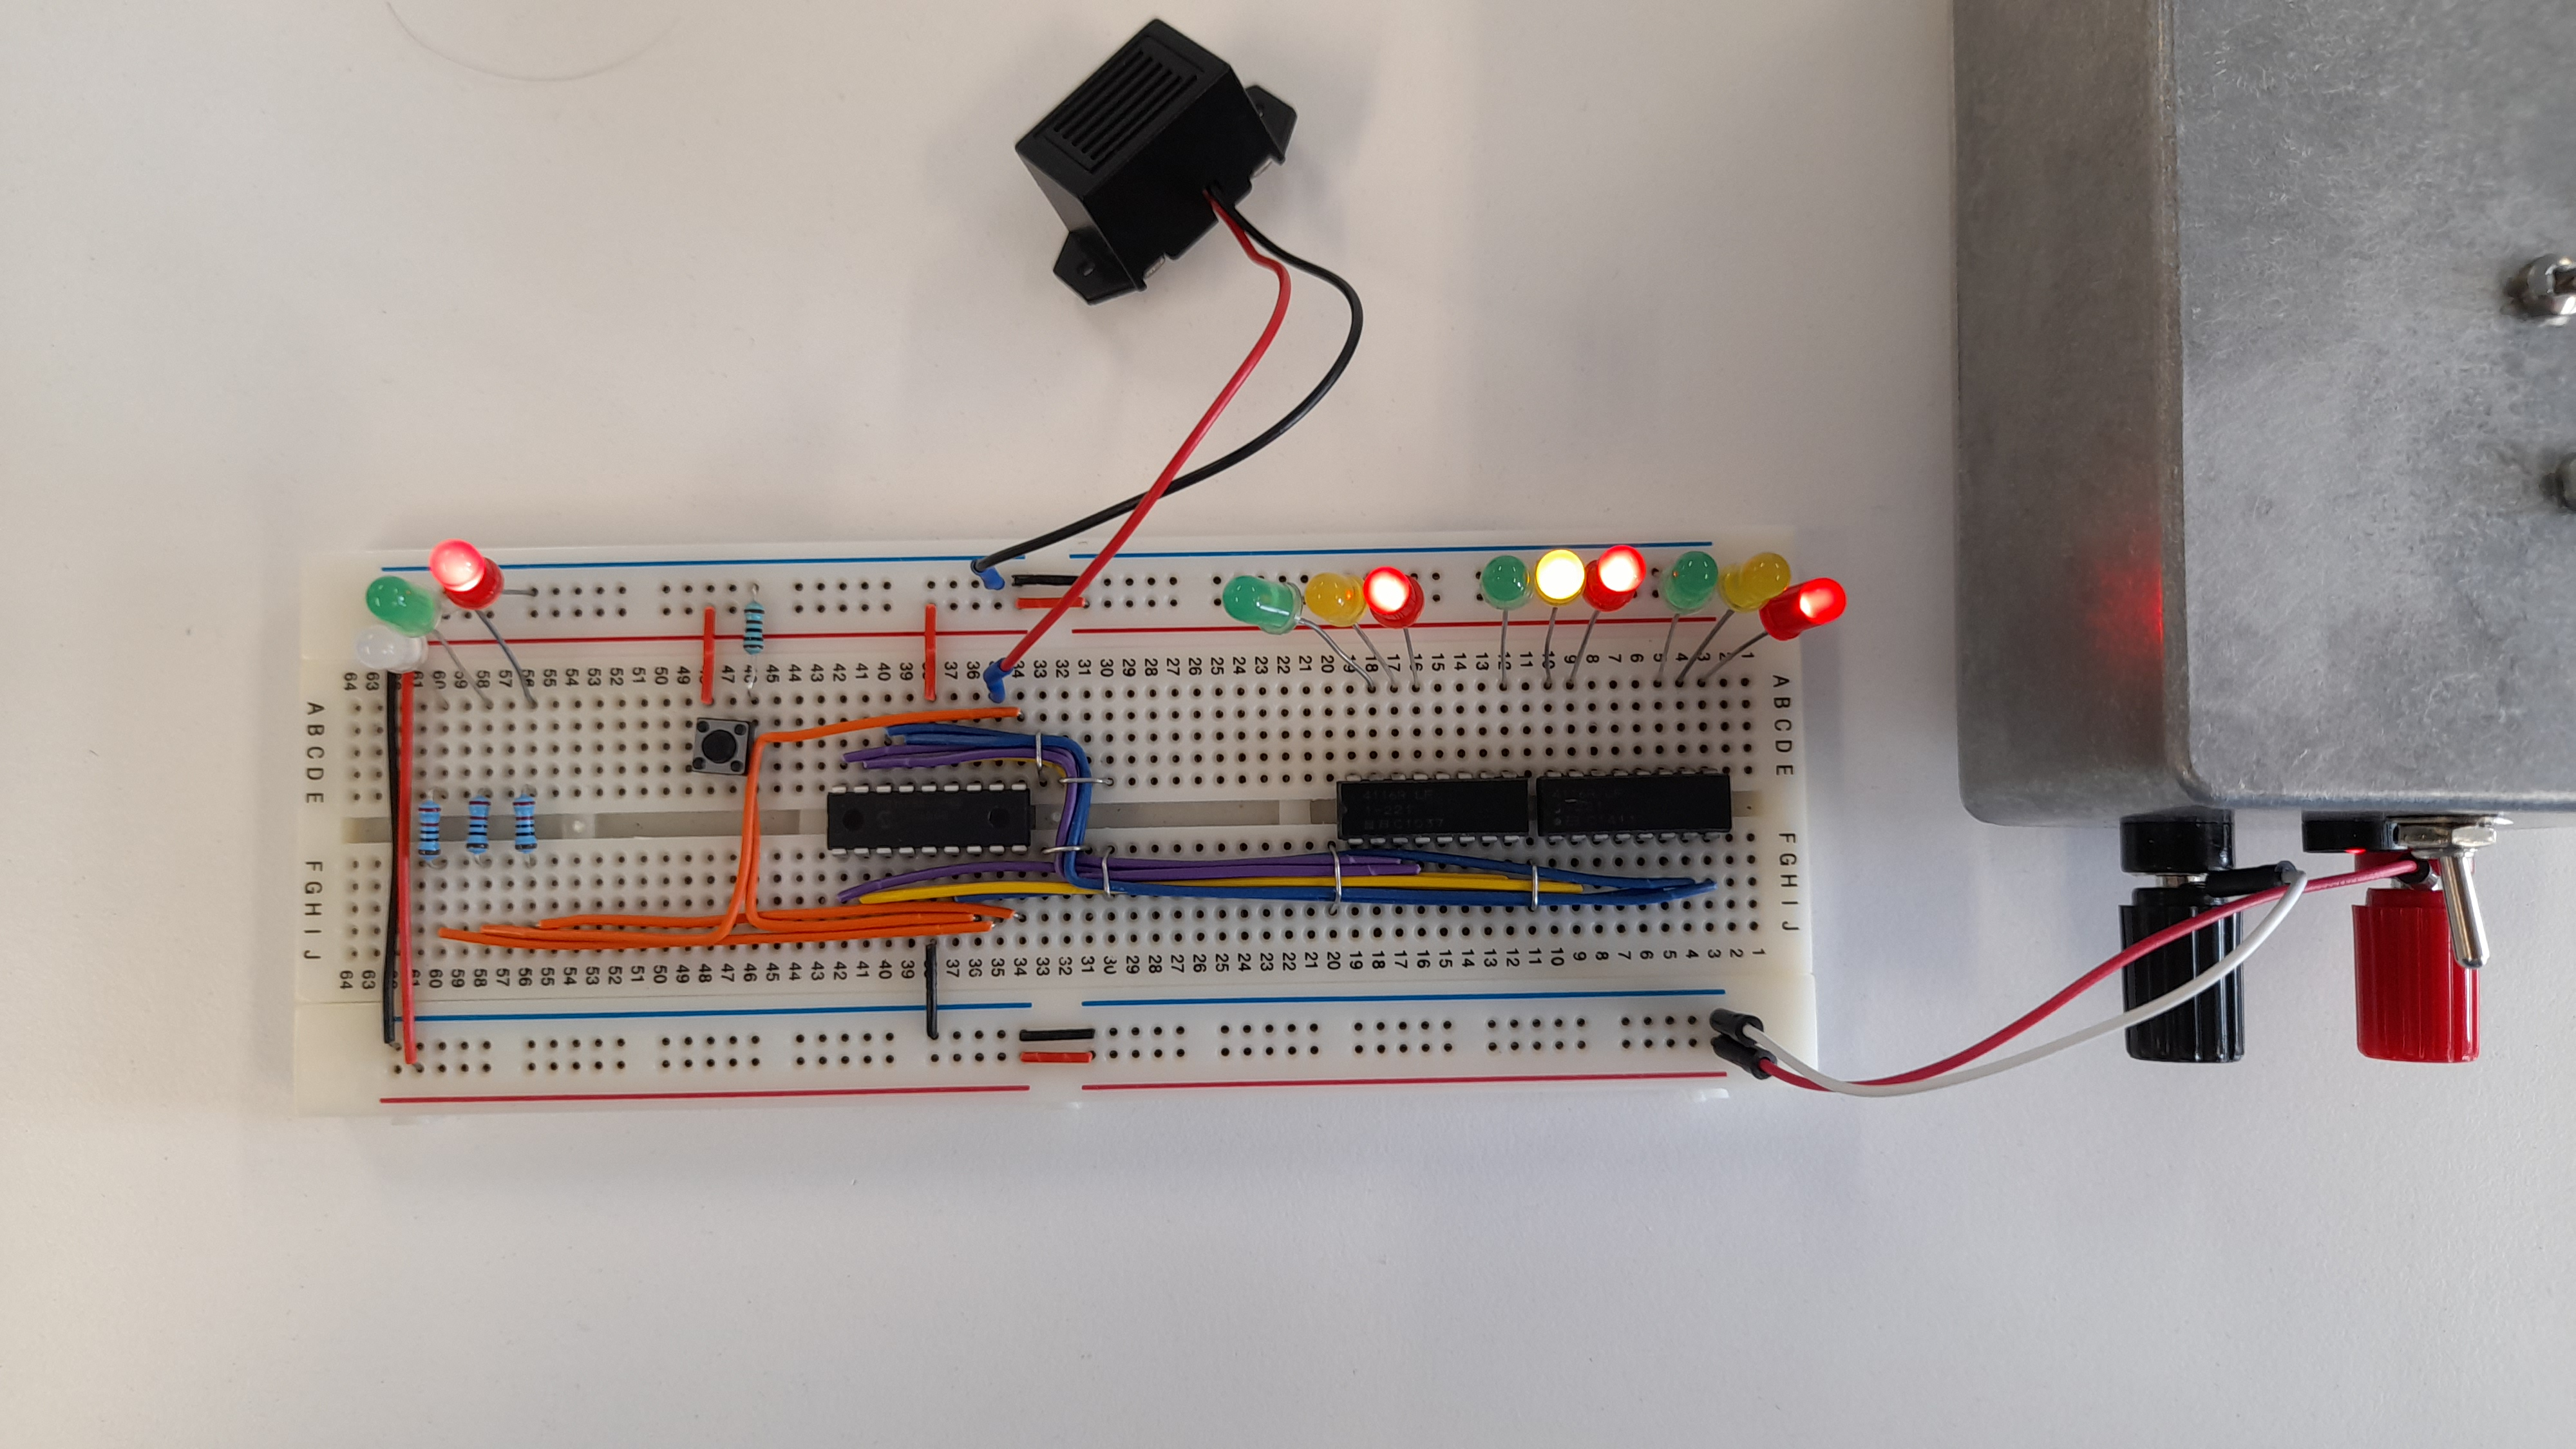
\includegraphics[width=0.9\textwidth]{images/final-testing/state_4.jpg}
        \caption{State 4 - green traffic lights in red and amber phase}
        \label{fig:state_4}
    \end{minipage}
\end{figure}
\begin{figure}[H]
    \begin{minipage}{0.45\textwidth}
        \centering
        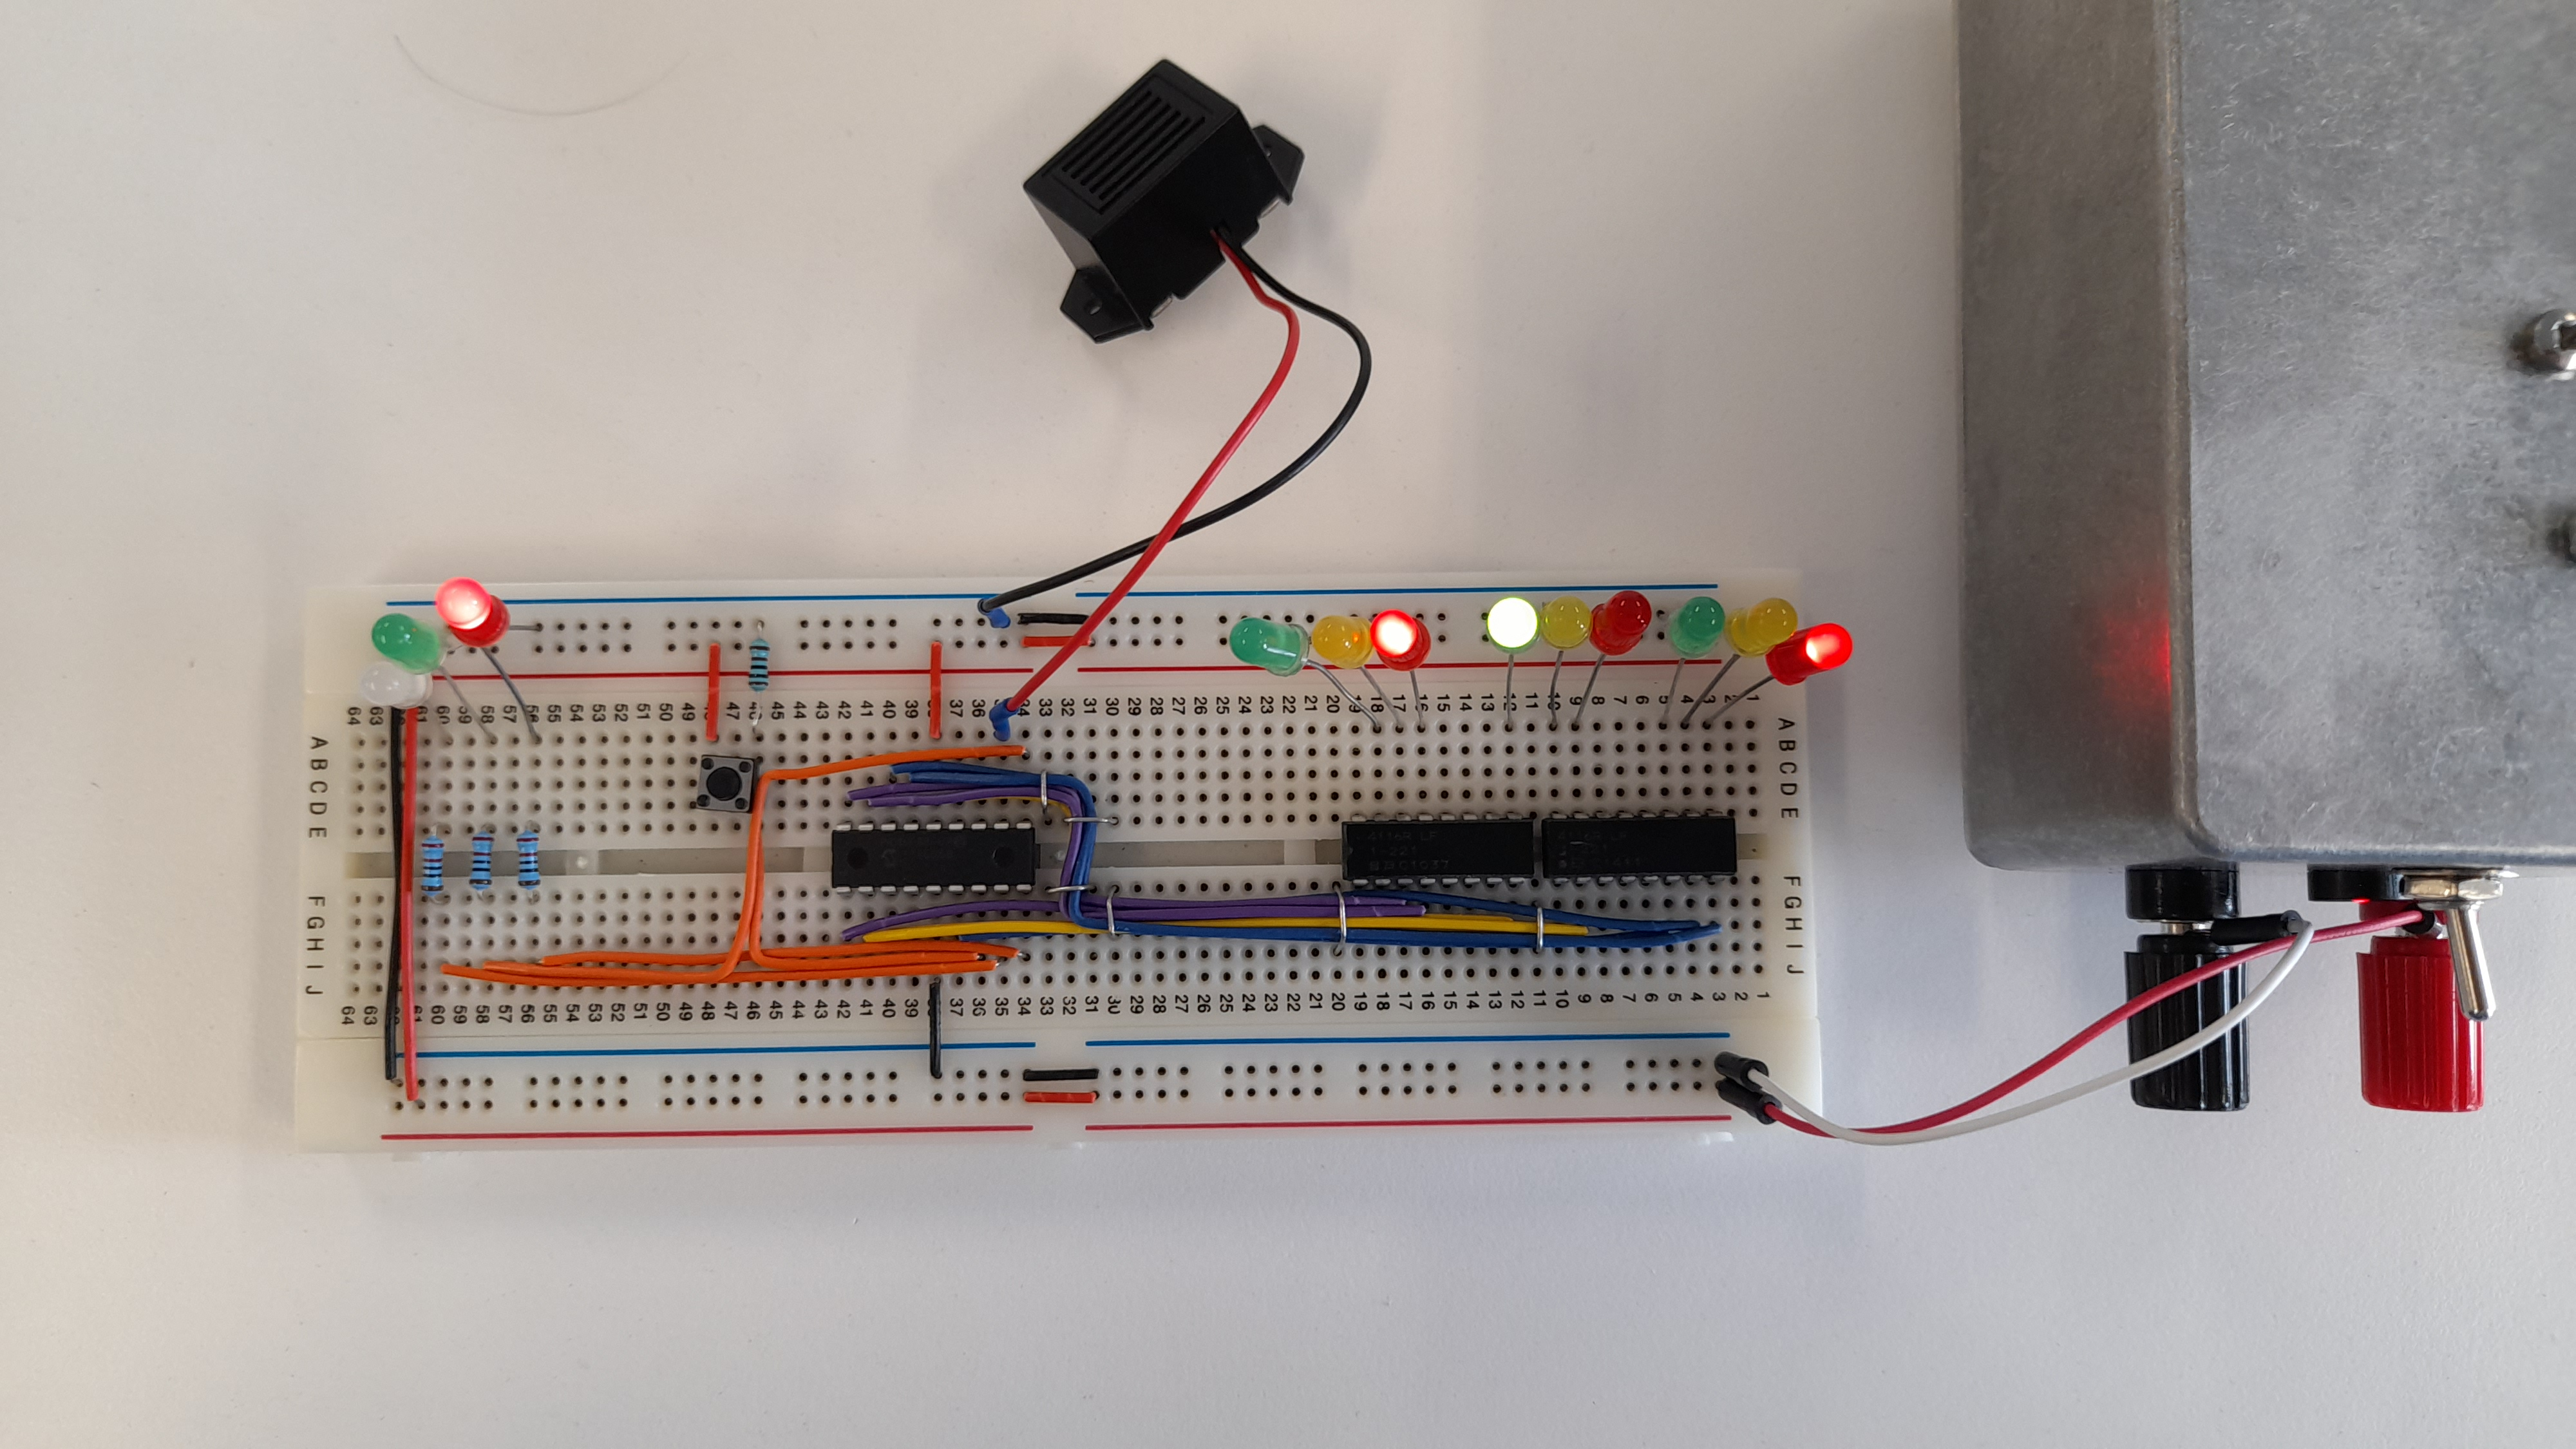
\includegraphics[width=0.9\textwidth]{images/final-testing/state_5.jpg}
        \caption{State 5 - green traffic lights in green phase}
        \label{fig:state_5}
    \end{minipage}\hfill
    \begin{minipage}{0.45\textwidth}
        \centering
        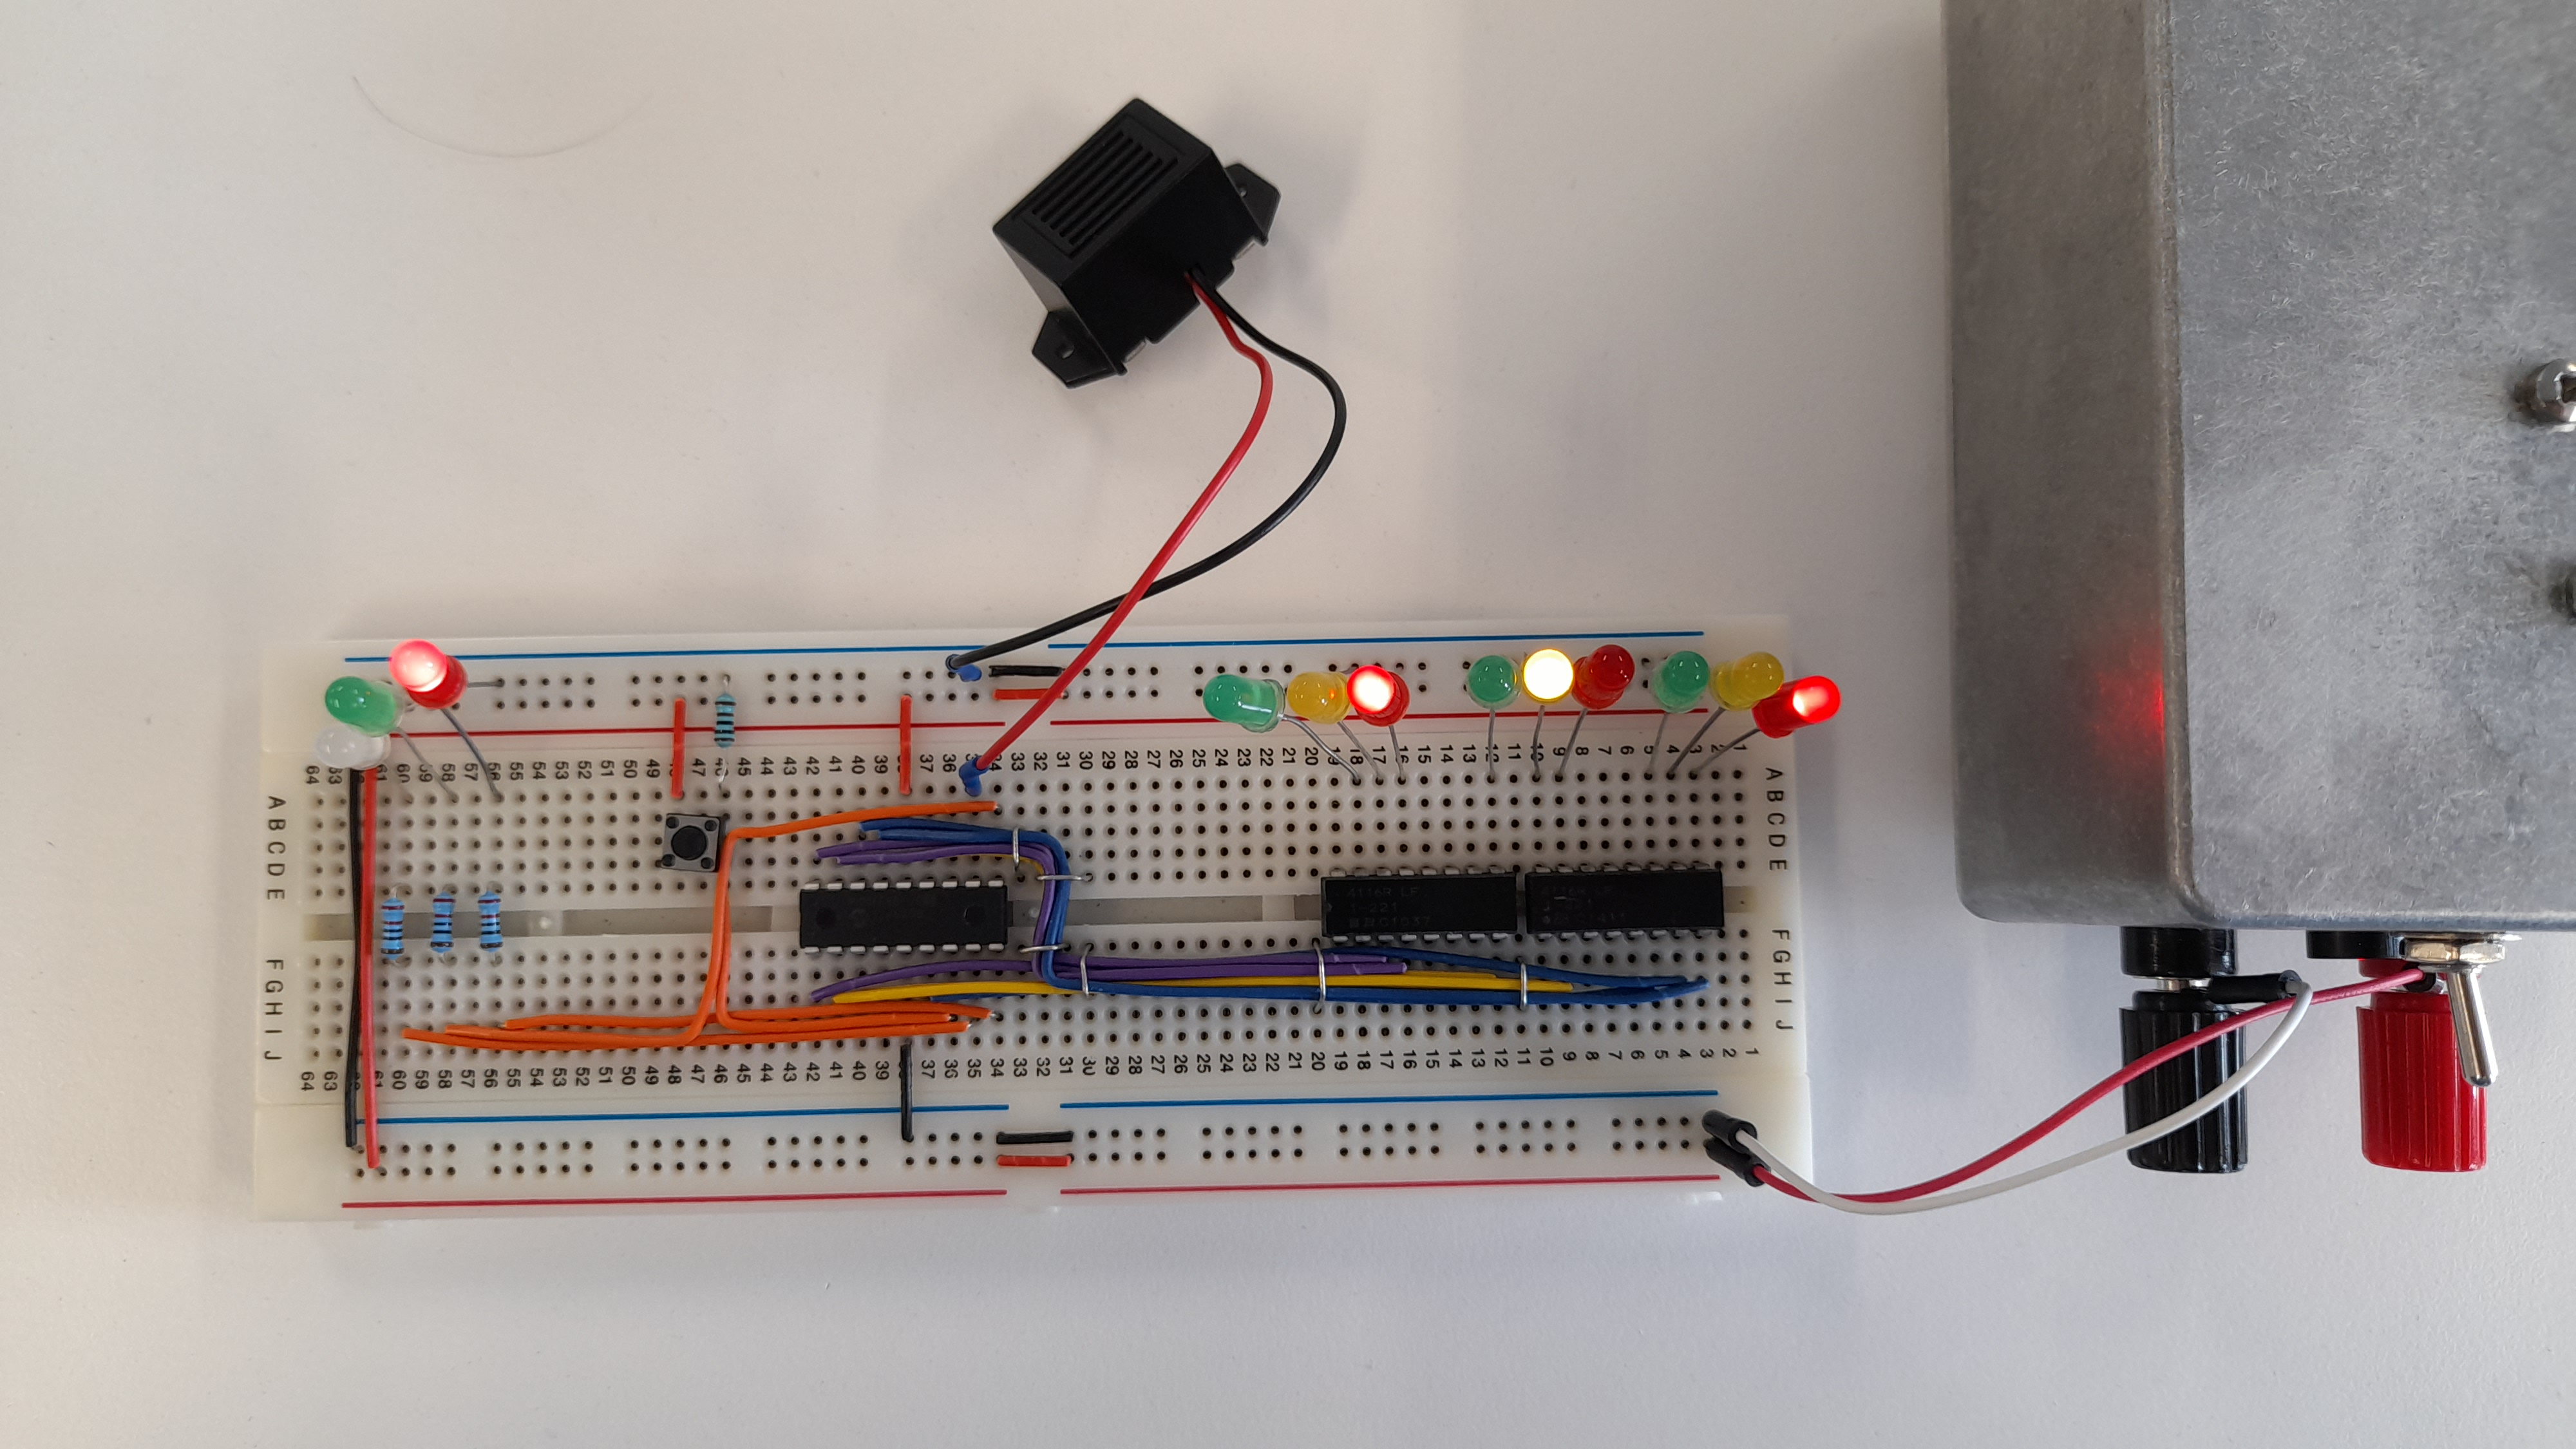
\includegraphics[width=0.9\textwidth]{images/final-testing/state_6.jpg}
        \caption{State 6 - green traffic lights in amber phase}
        \label{fig:state_6}
    \end{minipage}
\end{figure}
\begin{figure}[H]
    \begin{minipage}{0.45\textwidth}
        \centering
        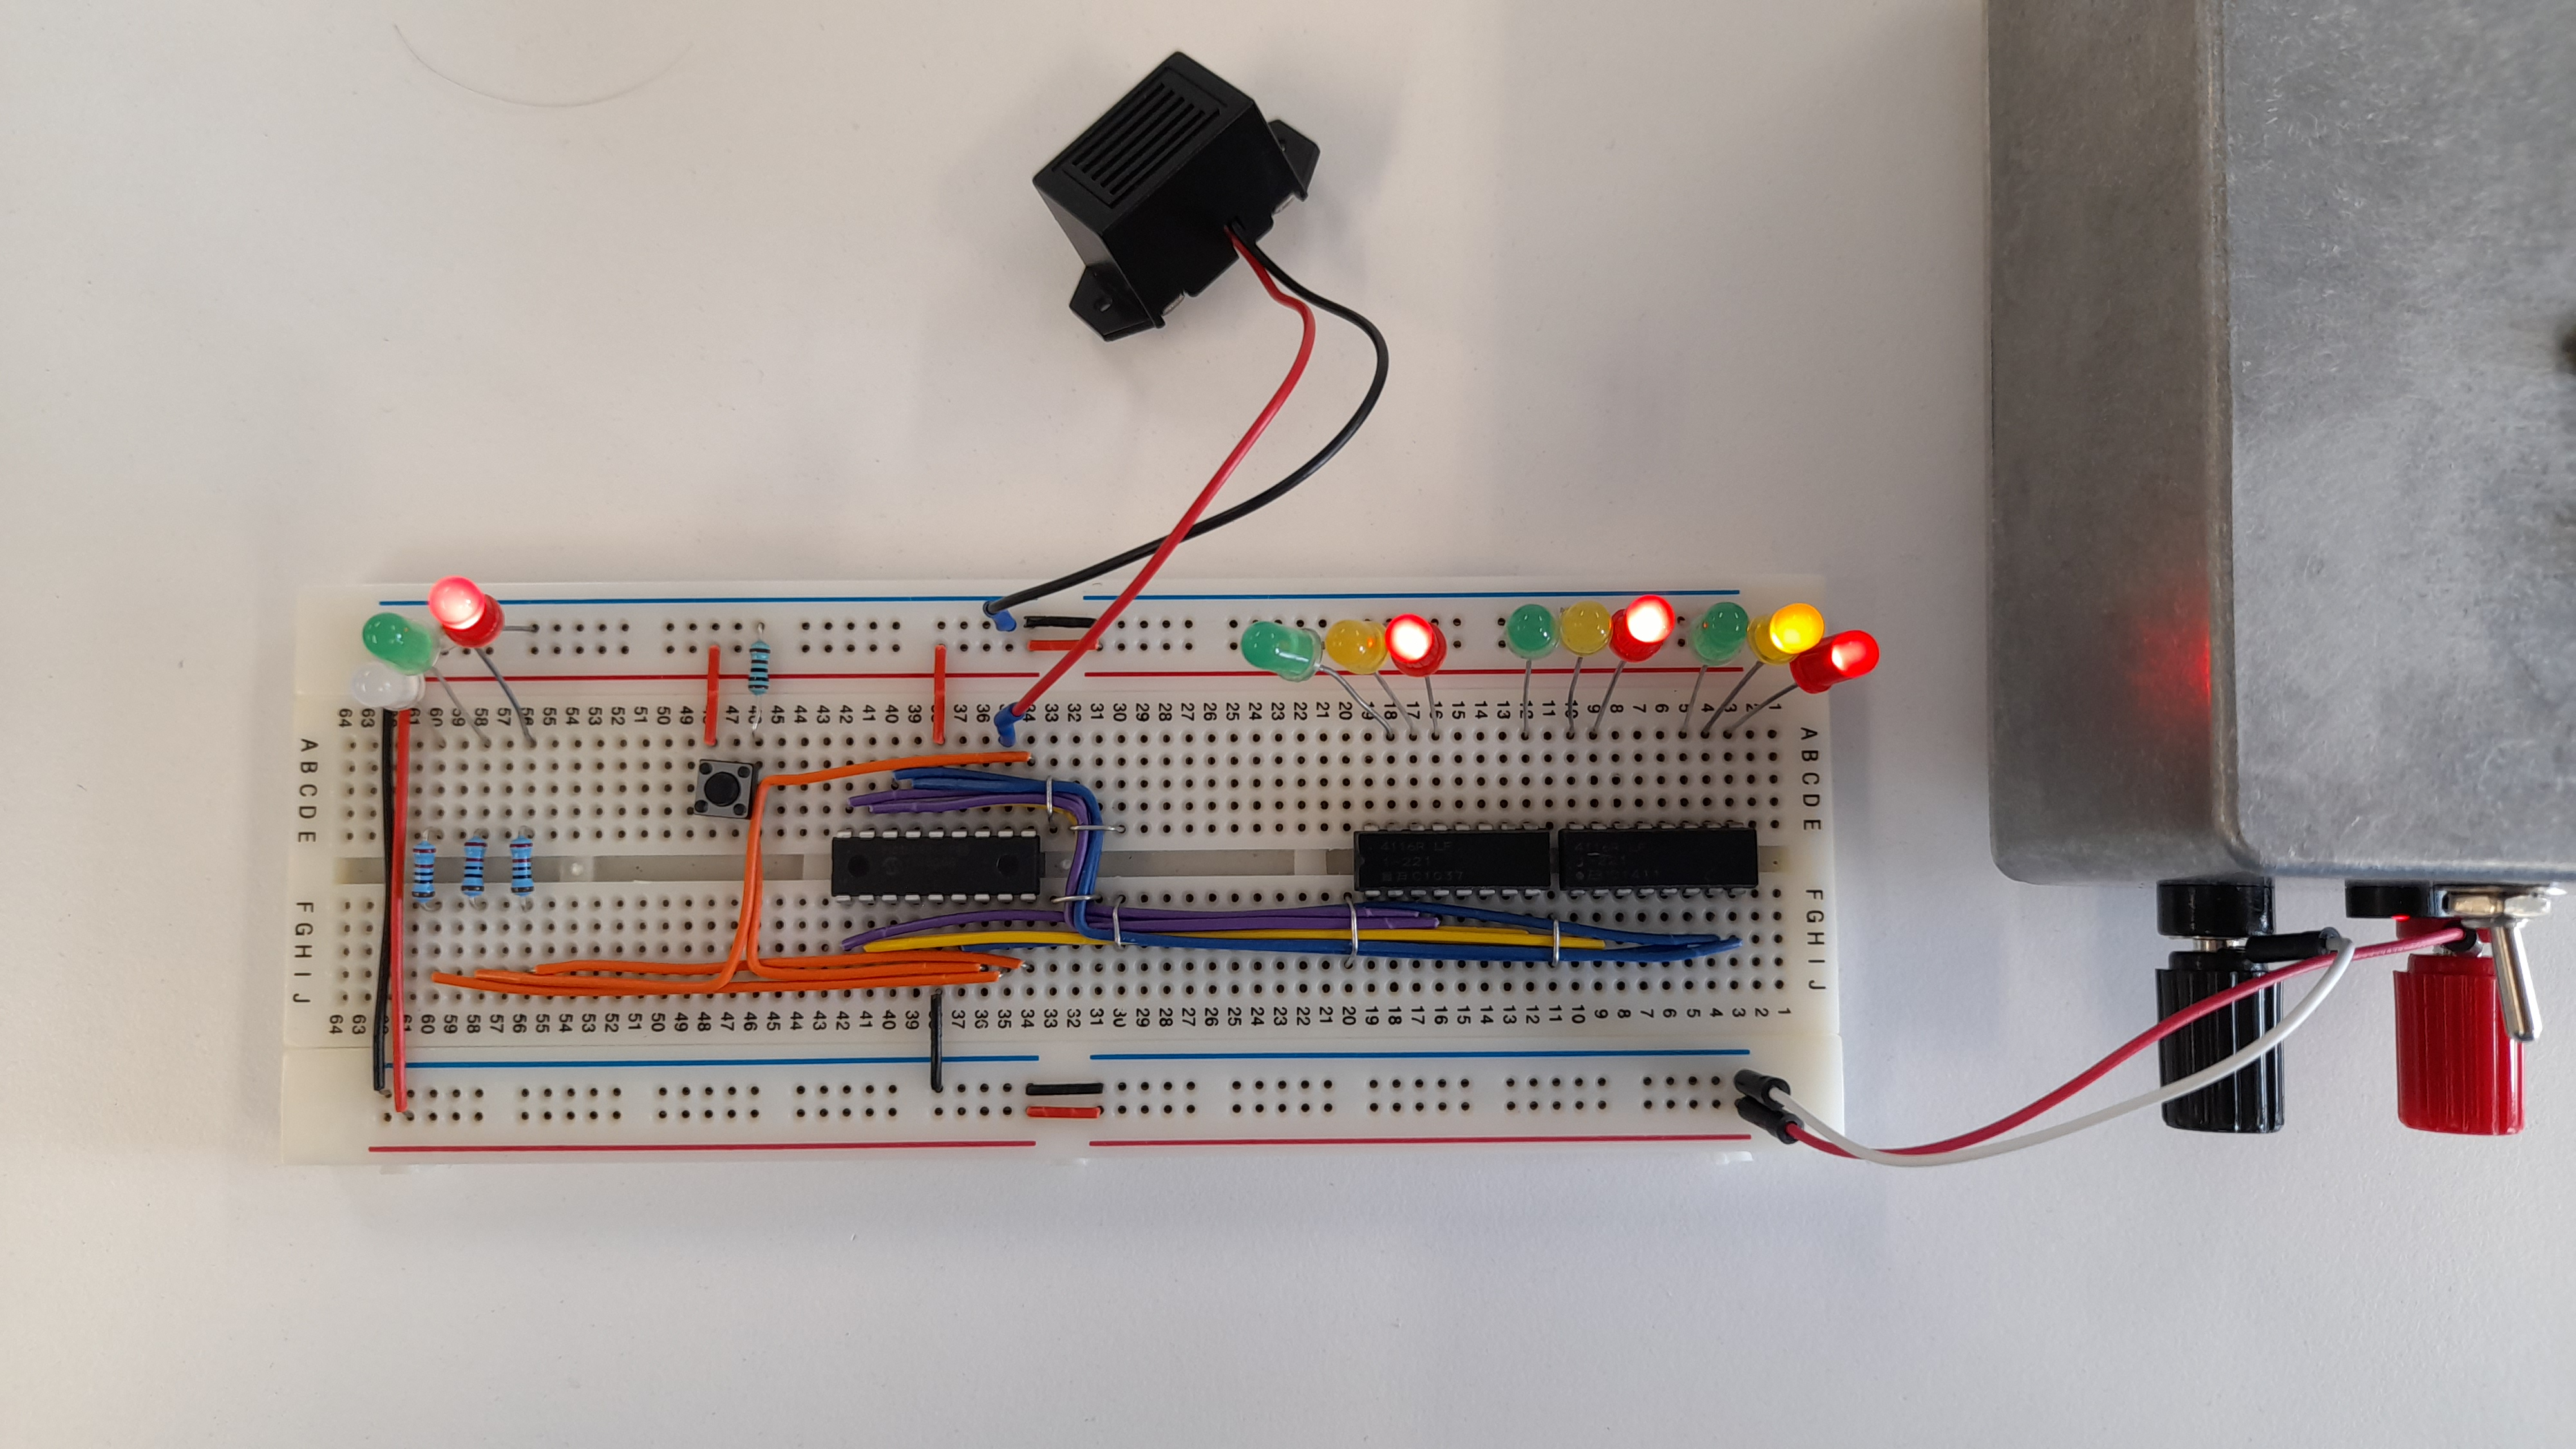
\includegraphics[width=0.9\textwidth]{images/final-testing/state_7.jpg}
        \caption{State 7 - blue traffic lights in red and amber phase}
        \label{fig:state_7}
    \end{minipage}\hfill
    \begin{minipage}{0.45\textwidth}
        \centering
        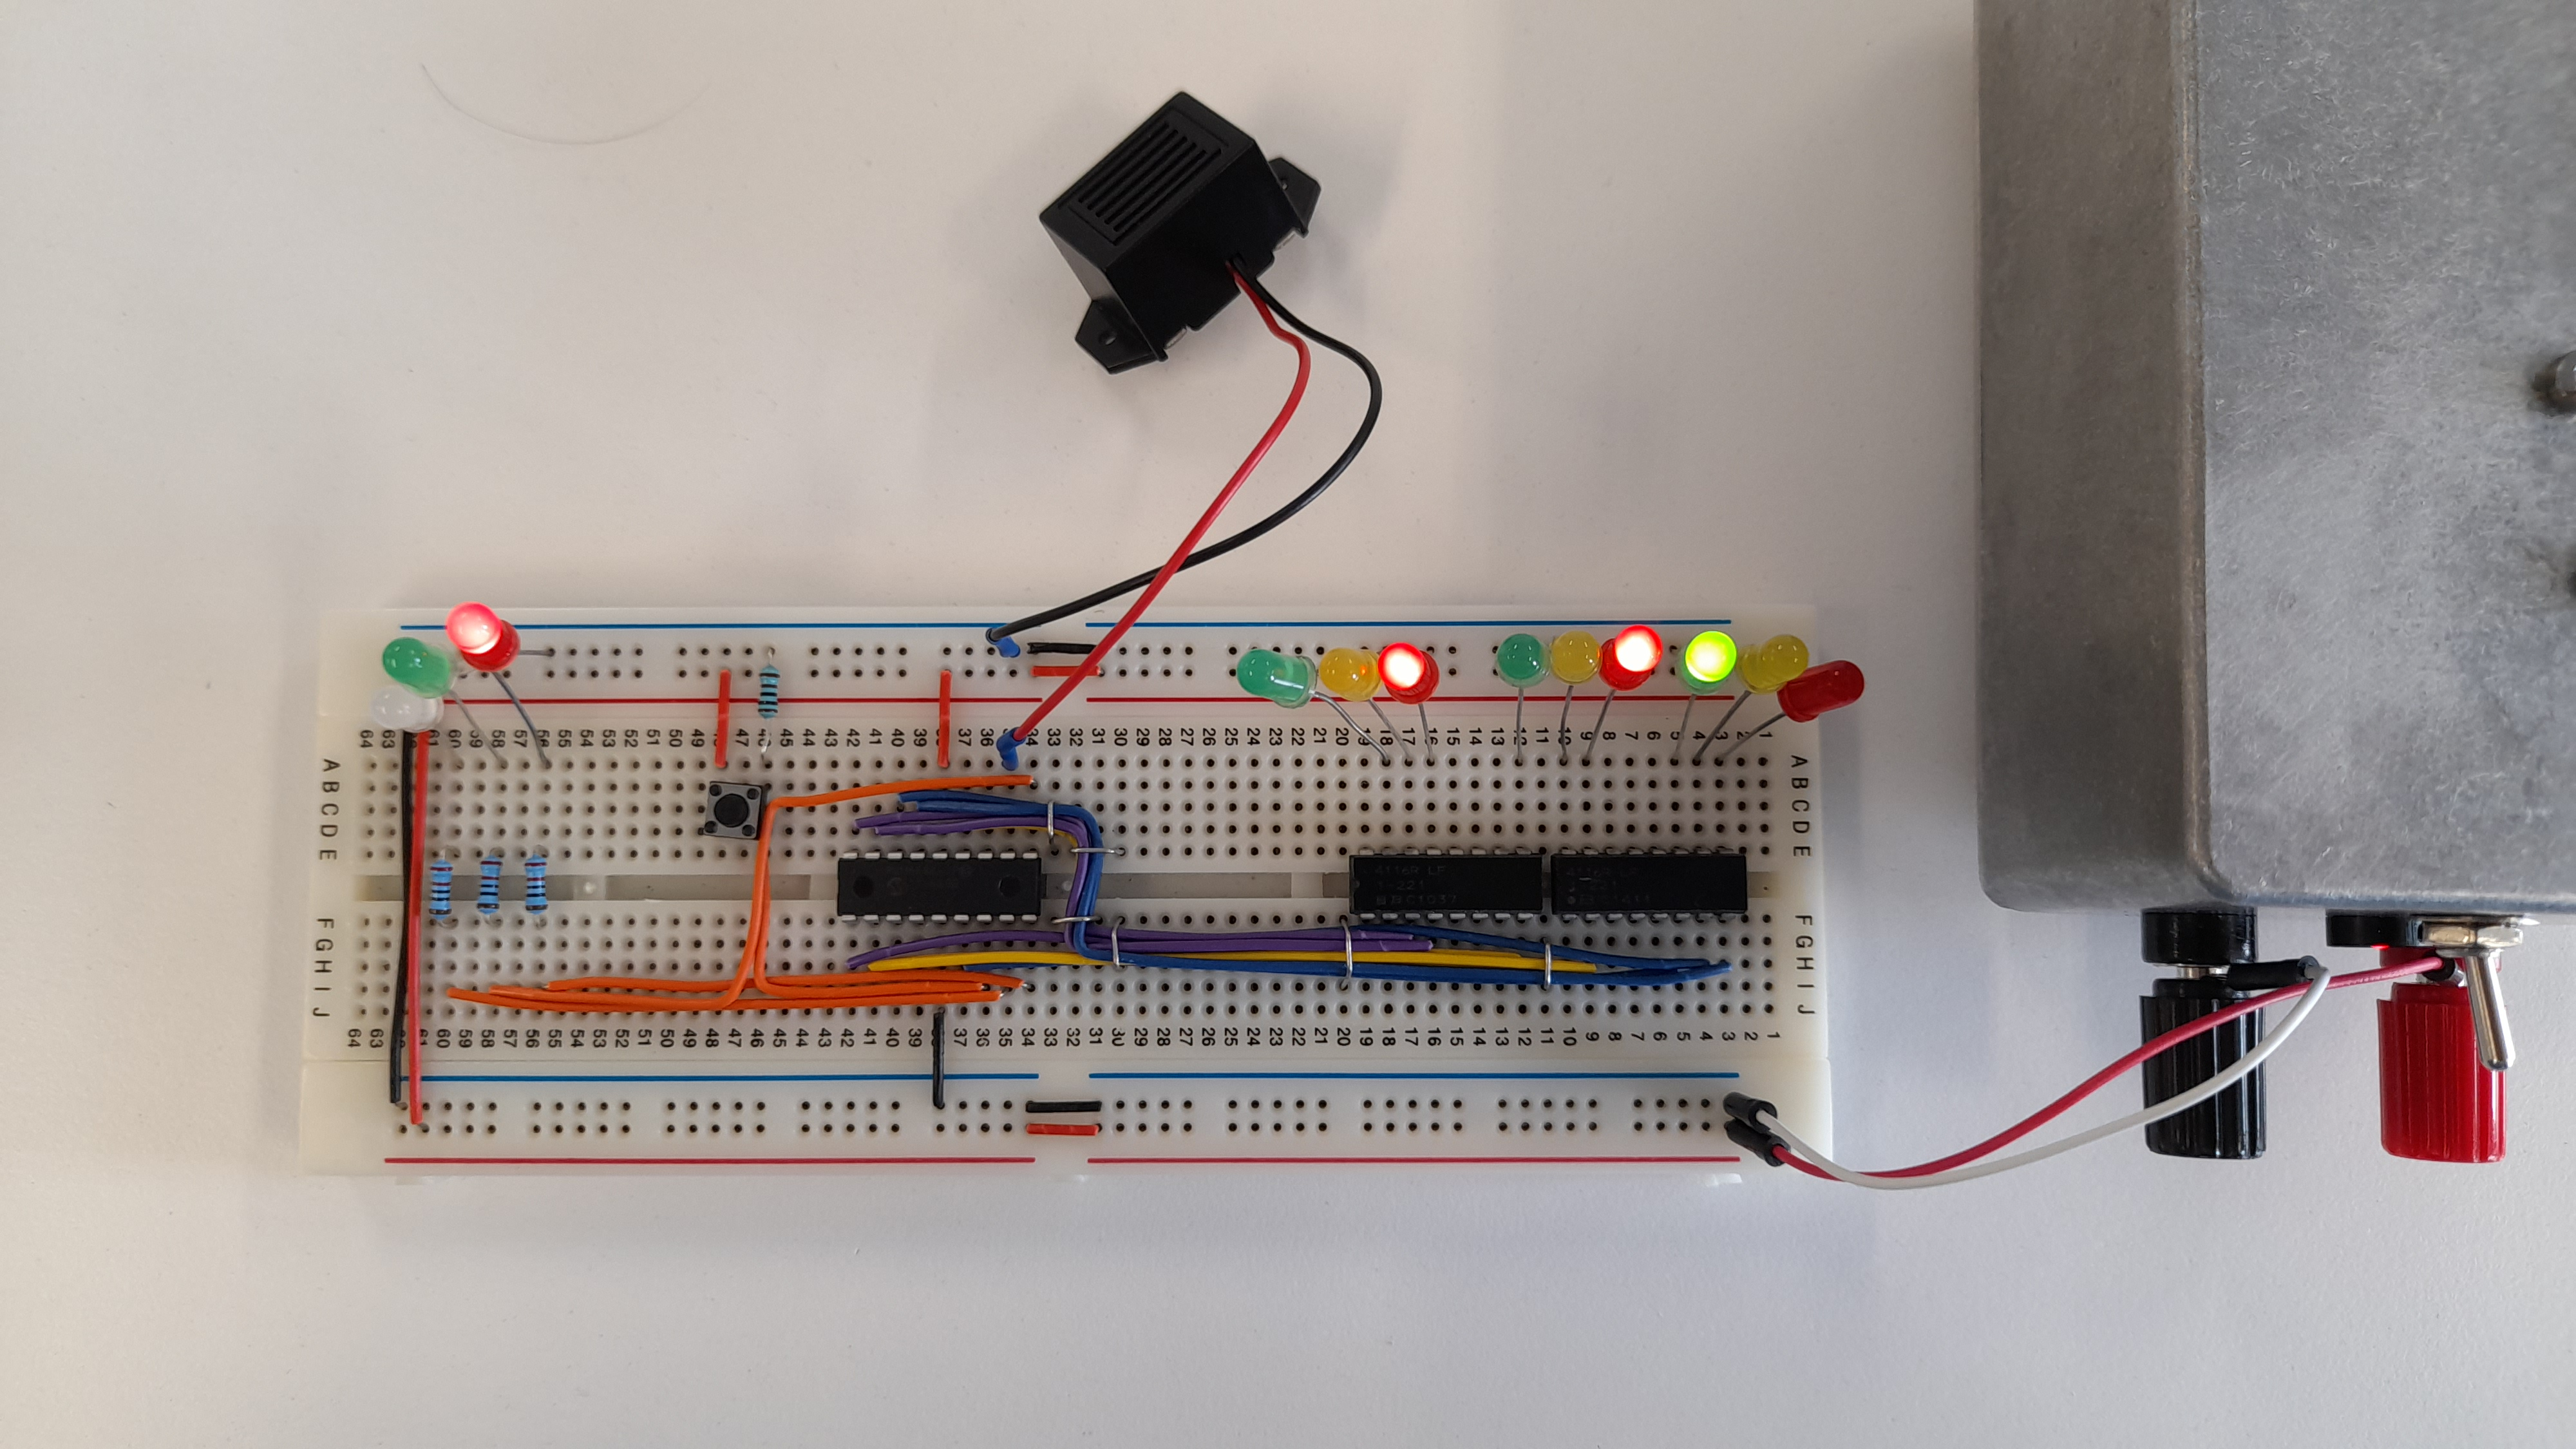
\includegraphics[width=0.9\textwidth]{images/final-testing/state_8.jpg}
        \caption{State 8 - blue traffic lights in green phase}
        \label{fig:state_8}
    \end{minipage}
\end{figure}
\begin{figure}[H]
    \begin{minipage}{0.45\textwidth}
        \centering
        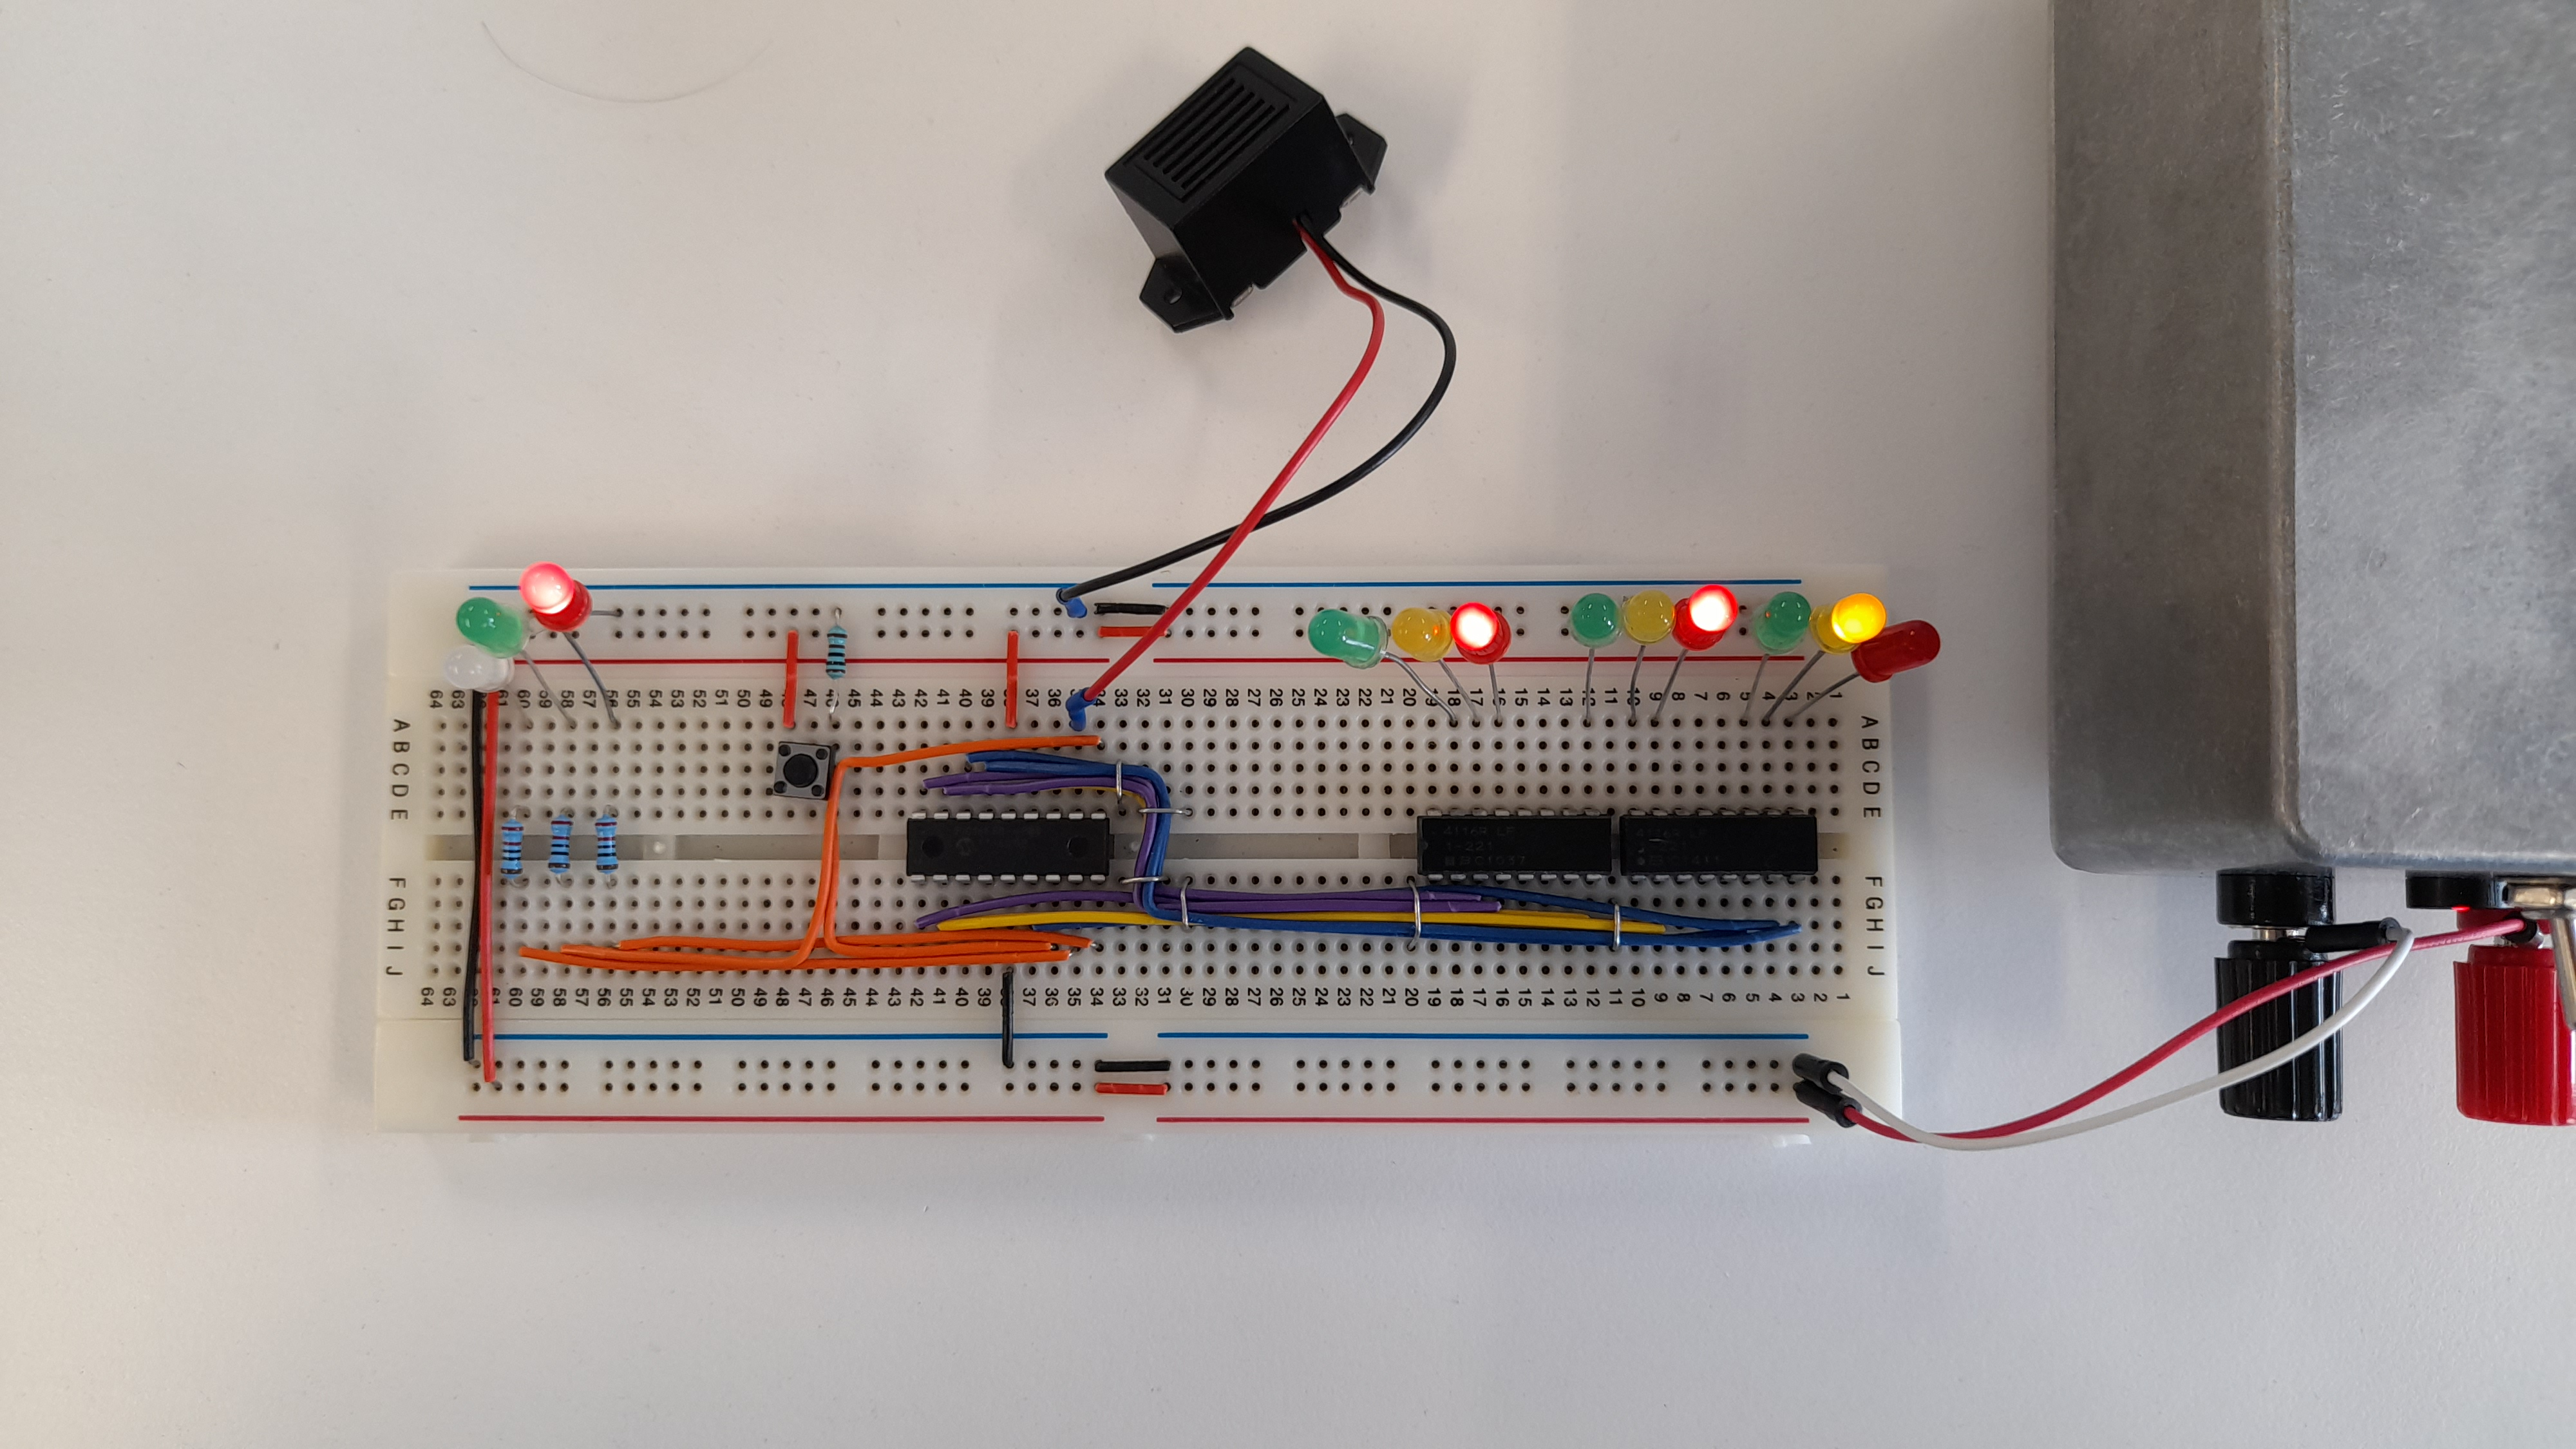
\includegraphics[width=0.9\textwidth]{images/final-testing/state_9.jpg}
        \caption{State 9 - blue traffic lights in amber phase}
        \label{fig:state_9}
    \end{minipage}\hfill
    \begin{minipage}{0.45\textwidth}
        \centering
        The system then loops back to state 1.
    \end{minipage}
\end{figure}

\subsection{Crossing Sequence}
\begin{figure}[H]
    \begin{minipage}{0.45\textwidth}
        \centering
        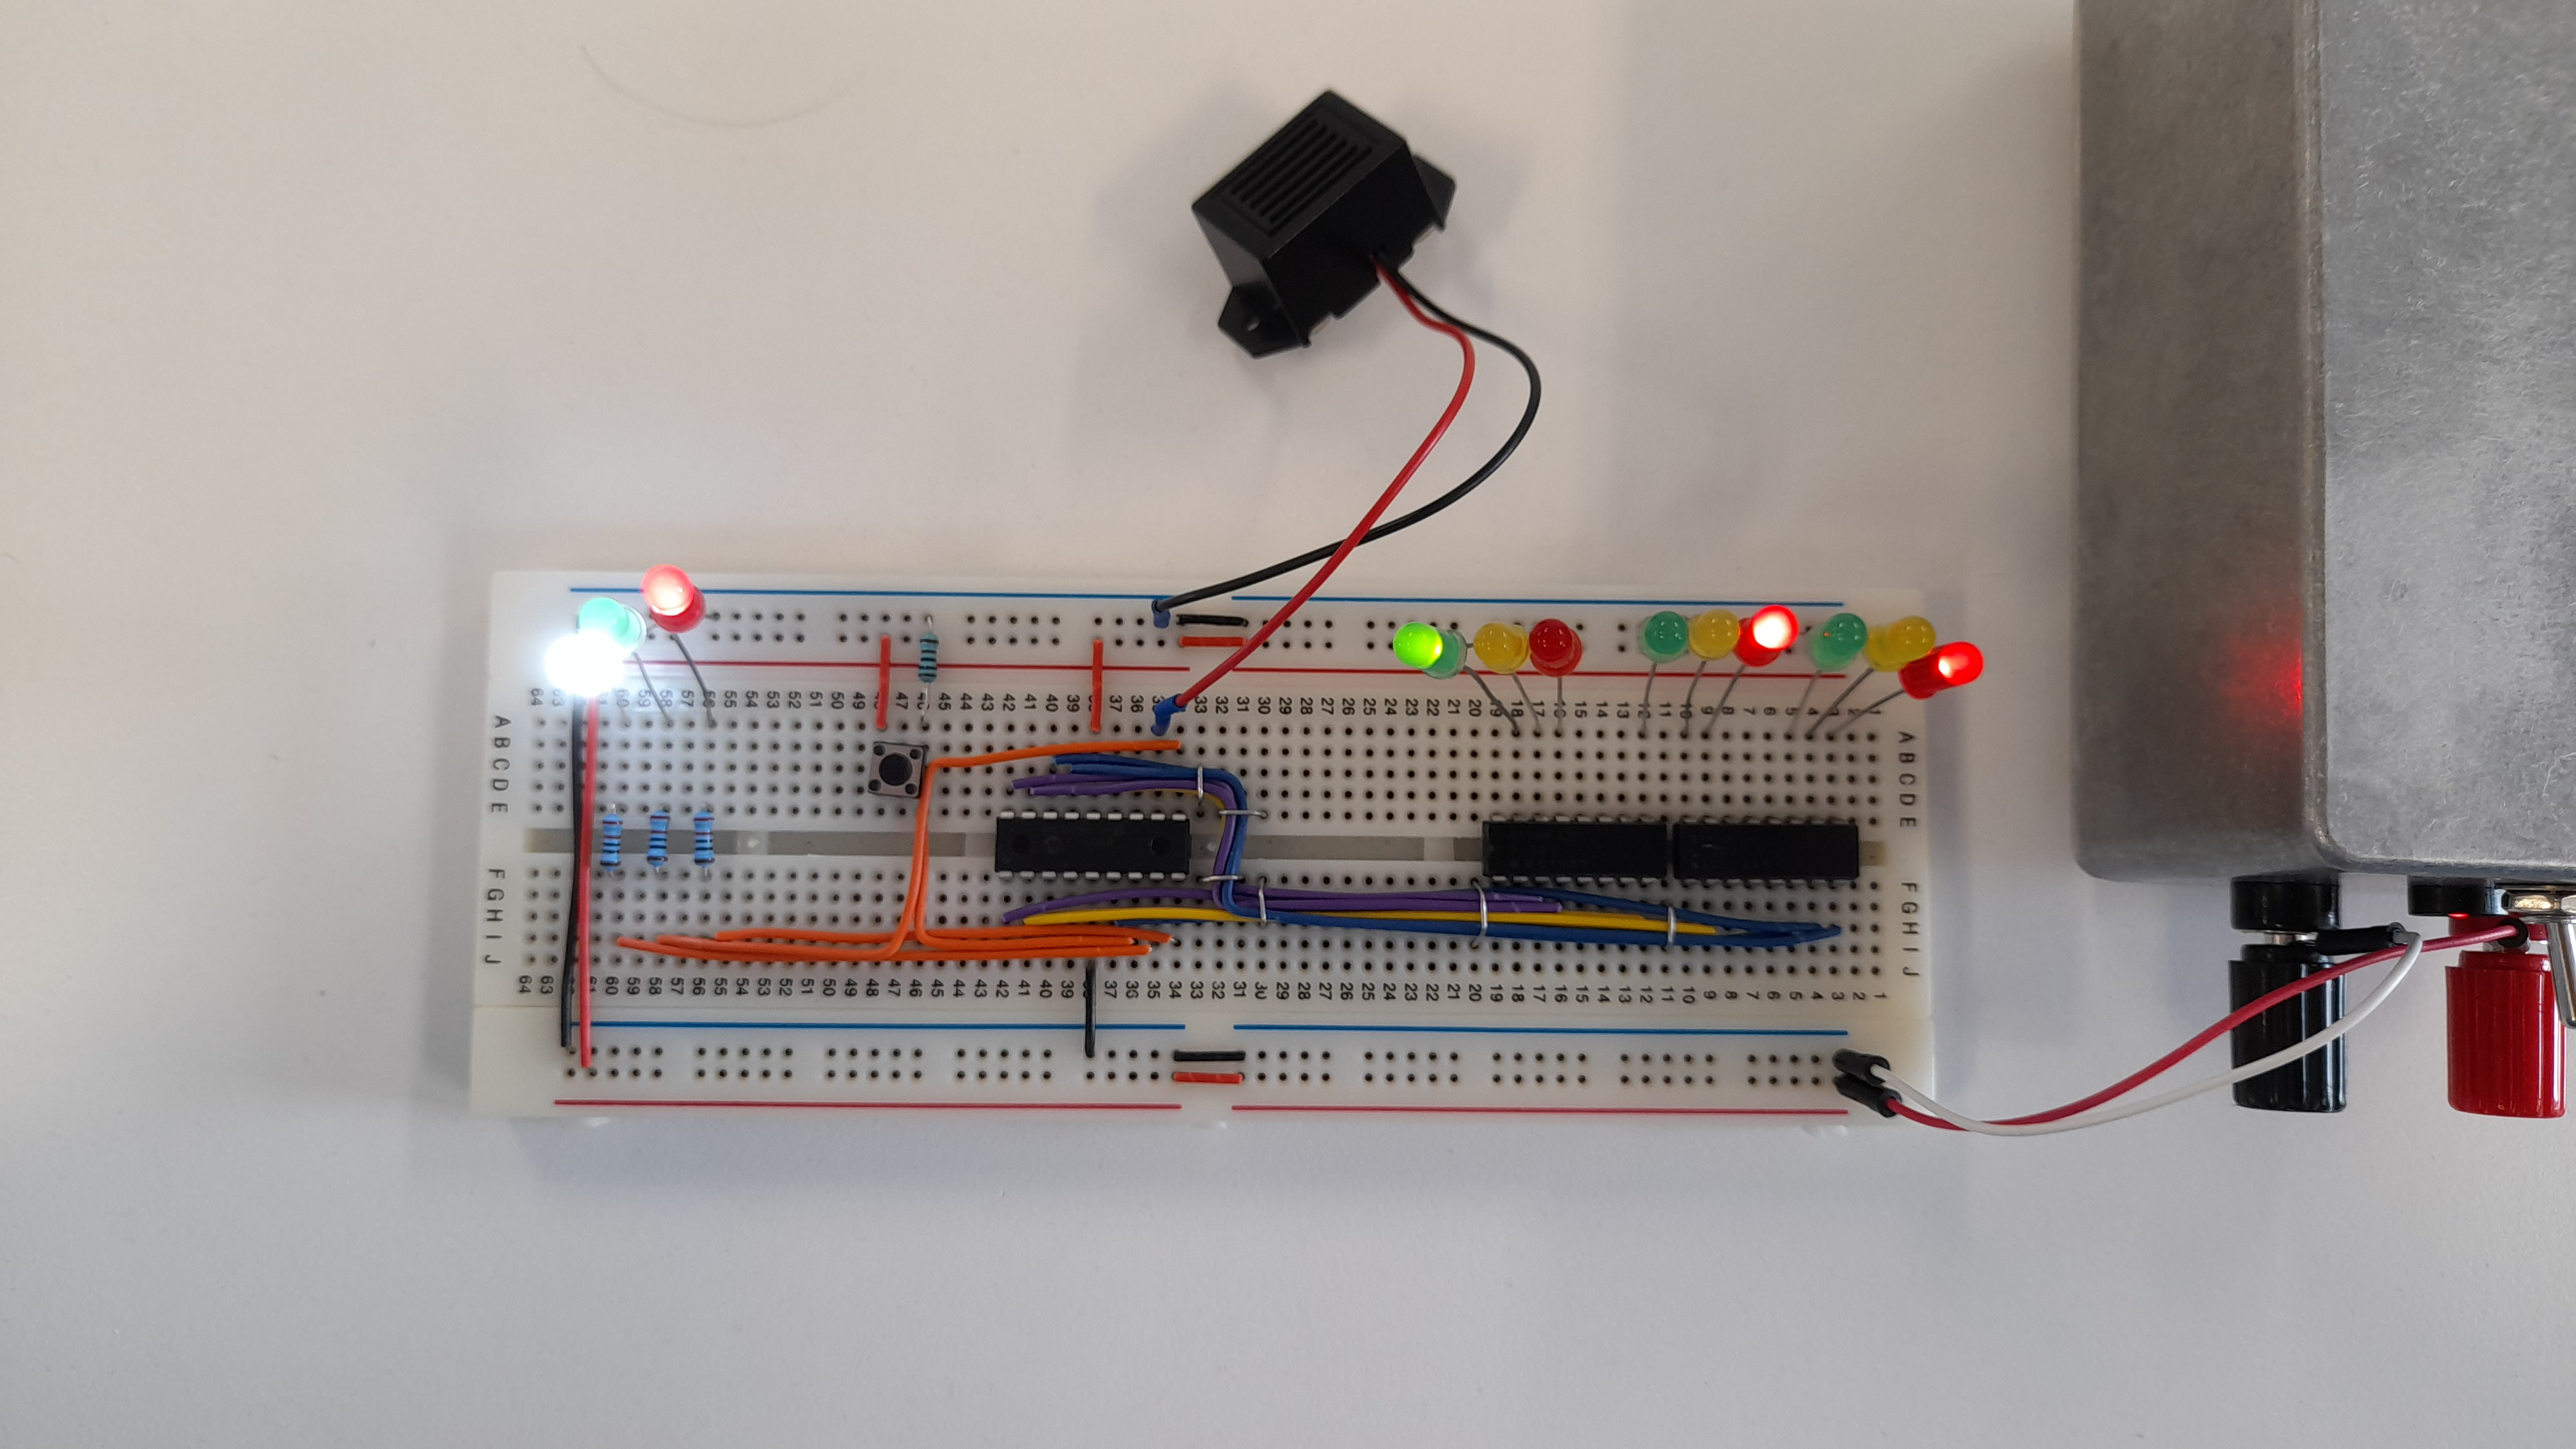
\includegraphics[width=0.9\textwidth]{images/final-testing/state_c_1.jpg}
        \caption{Crossing state 1 - wait button on phase}
        \label{fig:state_c_1}
    \end{minipage}\hfill
    \begin{minipage}{0.45\textwidth}
        \centering
        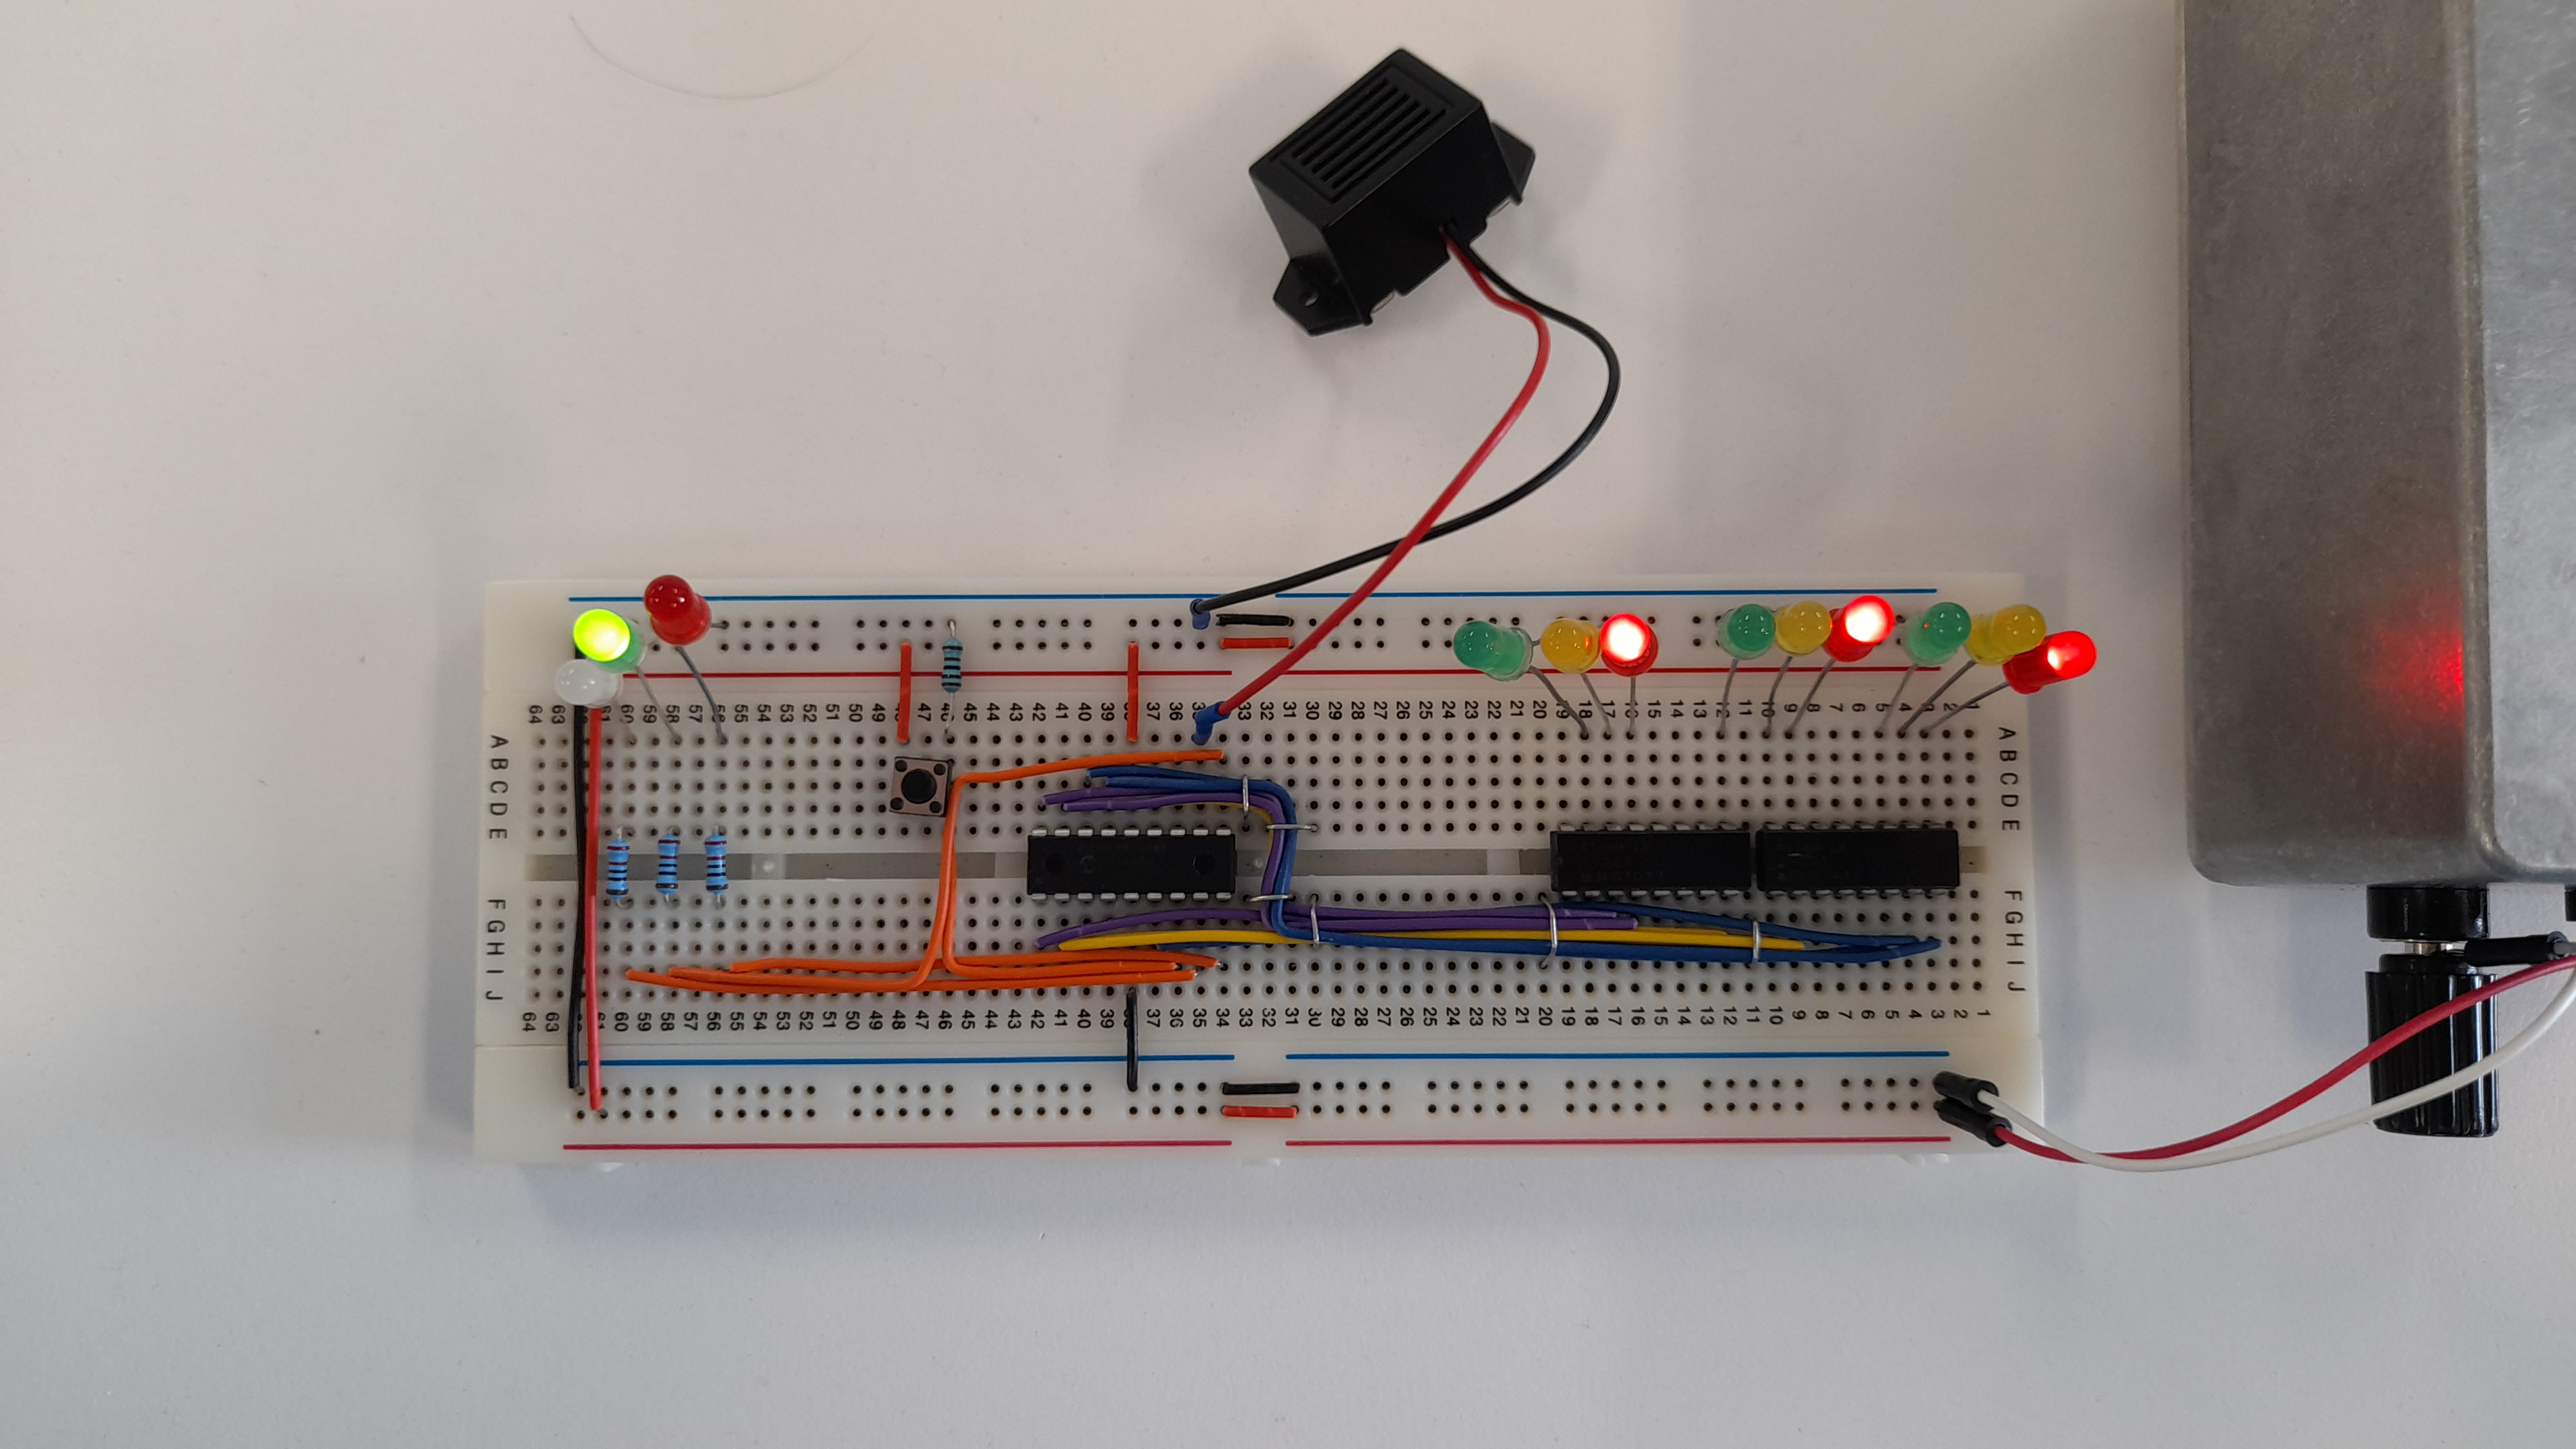
\includegraphics[width=0.9\textwidth]{images/final-testing/state_c_2.jpg}
        \caption{Crossing state 2 - safe to cross phase}
        \label{fig:state_c_2}
    \end{minipage}
\end{figure}